\documentclass[12pt,prb,aps,epsf]{article}
\usepackage[utf8]{inputenc}

\title{LP20 - Conversion de puissance}
\author{Guitara de Marietta Ubero Gonzalez}
\date{Agrégation 2019}

\usepackage{natbib}
\usepackage{graphicx}
\usepackage{amsmath}
\usepackage[a4paper, total={6in, 8in}]{geometry}
\usepackage{xcolor}

\geometry{hmargin=2cm,vmargin=2cm}

\begin{document}

\maketitle

\tableofcontents

\section*{Pré-requis}
\begin{itemize}
    \item Electromagnétisme 
    \item Induction
    \item mécanique
\end{itemize}



\section*{Introduction}
L'étude du phénomène d'induction électromagnétique met en évidence la possibilité de convertir de l'énergie électrique en énergie mécanique et réciproquement. Des nombreuses applicatuions sont basées sur ce phénomène.\medskip

\textcolor{red}{Dates historiques}

\section{Principe de la conversion électromécanique}



\subsection{Rails de Laplace}

Le dispositif étudié  comprend deux rails parallèles dans un plan horizontal, conducteurs et distants de $L$. On place sur ceux-ci une tige mobile conductrice $NM$. L'ensemble est placé dans un champ magnétique uniforme et constant.

\begin{center}
    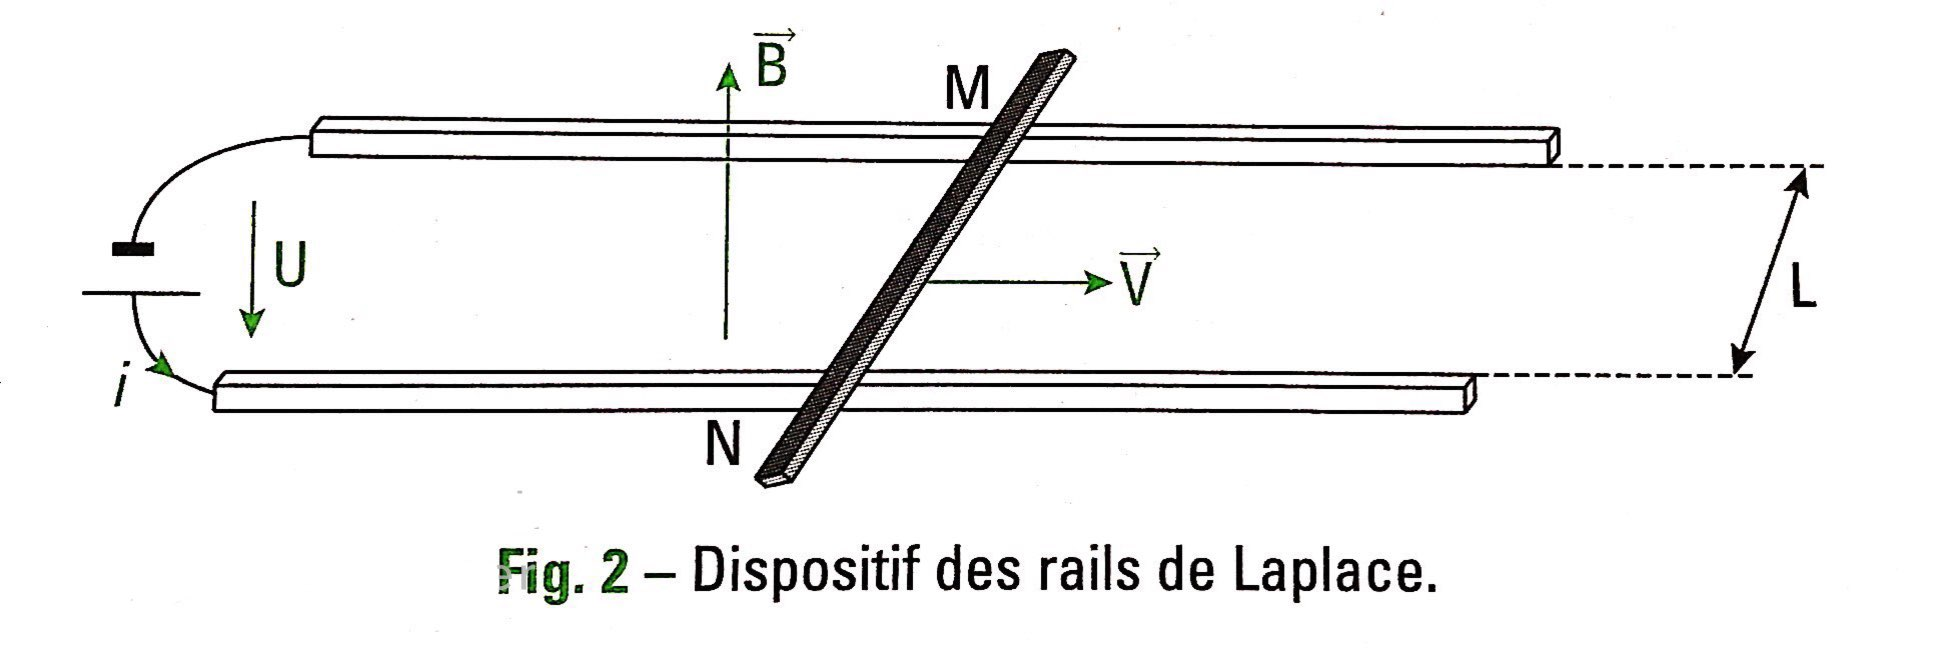
\includegraphics[scale=0.18]{railslaplace.jpg}
\end{center}

Considerons un conducteur électrique dans lequel les porteurs de charges sont des électrons de charge notée $-q$. En conservant l'hypothèse du champ magnétique constant et en notant que la barre se déplace à la vitesse $\vec{V}$ par rapport au référentiel $R$ lié au laboratoire. Exprimons la puissance $P$ de la force $\vec{f}=(-q(\vec{v} + \vec{V}) \land \vec{B})$ exercée sur les porteurs, qui se déplacent à la vitesse $\vec{v}$ :
\begin{eqnarray}
    P &=& \vec{f} \cdot (\vec{v} + \vec{V}) = (-q(\vec{v} + \vec{V})\land \vec{B} ) (\vec{v} + \vec{V}) = 0\\
 &=& -q ( \vec{v}  \land \vec{B} ) \cdot \vec{v} -q( \vec{v}  \land \vec{B} ) \cdot \vec{V} -q ( \vec{V}  \land \vec{B} ) \cdot \vec{v} -q ( \vec{V}  \land \vec{B} ) \cdot \vec{V}\\
     &=& -q (\vec{v}  \land \vec{B} ) \cdot \vec{V} -q ( \vec{V}  \land \vec{B} ) \cdot \vec{v}
\end{eqnarray}

Le premier terme de l'expression de la puissance, représente la puissance d'une force $\vec{F_L} = -q \vec{v} \land \vec{B} $ orthogonale au plan formé par les vecteurs $\vec{v}$ et $\vec{B}$ : elle est donc colinéaire à $\vec{V}$. Cependant, les porteurs de charges sont liés au réseau cristallin qui constitue le conducteur mobile et ils ne peuvent donc pas s'extraire de ce dernier. Par conséquent, la quantité de mouvement associée à $\vec{F_L}$ est transférée au réseau. Ce bilan donne lieu au mouvement macroscopique du conducteur. Ce mouvement est dû à la force de Laplace. On peut ainsi dire qu'il y a eu transfert d'une \textbf{énergie de nature électrique} (associé au mouvement des porteurs de charges mobiles) en une \textbf{énergie de nature mécanique}; c'est la \textbf{conversion électromécanique de puissance}. \medskip

Le second terme de l'expression de la puissance représente la puissance d'une force qui est dans ce cas dirigée selon l'axe du conducteur; elle met en mouvement les porteurs de charge et donne ainsi lieu à une puissance de nature électrique. Il convient à nouveau de noter que c'est un transfert d'énergie car $-q\vec{V}\land \vec{B}$ est une force due au mouvement mécanique de la tige. Il y a donc transfert de \textbf{l'énergie de nature mécanique} en \textbf{énergie de nature électrique}. C'est donc une conversion électromécanique de puissance.\medskip

\textcolor{green}{Dans le second terme de la puissance on voit apparaître $\vec{E_m}=\vec{V} \land \vec{B}$}

Le bilan complet s'écrit alors :
\begin{equation}
    P_m + P_e = 0
\end{equation}

Cette équation résume ainsi la conversion électromécanique de la puissance ayant lieu à chaque instant, puisque $P_m = - P_e$. En autres termes, la puissance mécanique créée provient de la puissance électrique $-P_e$ perdue par les porteurs de charges. Elle traduit en outre la conservation de l'énergie.\medskip

Nous pouvons alors distinguer deux types de fonctionnement :

\begin{itemize}
    \item Générateur : conversion de la puissance mécanique en puissance électrique.
    \item Moteur : conversion de la puissance électrique en mécanique
\end{itemize}

\section{Machine à courant continu}
Les machines à courant continu font partie des convertisseurs électro-magnéto-mécanique réversibles. Elles ont été les premières à être utilisées massivement dans toutes les gammes de puissance du fait de la simplicité de leur commande en vitesse.\medskip

Cependant, leur principe de fonctionnement nécessite un contact glissant entre la partie mobile et la partie fixe, qui, dans le cas d'une machine à entrefer radial, est réalisé grâce à un système \textbf{collecteur-balais}. Ce système qui constitue une limitation en vitesse de rotation et en puissance développée, est sujet à l'usure et nécessite un entretien régulier.\medskip

Actuellement, malgré la concurrance des machines à courant alternatif munies de leur commande électronique, les machines à courant continue restent néanmoins encore très présentes et utilisées dans une gamme de puissance allant, pour les moteurs de traction, jusqu'à quelques centaines de kilowatts.\medskip


\subsection{Structure et principe de fonctionnement}

Avant de décrire le principe de fonctionnement de cette machine, définissons dans ce qui suit, ses principaux éléments.\medskip

\begin{itemize}
    \item Circuits éléctriques
    \begin{itemize}
        \item \textbf{L'induit :} circuit élctrique soumis au champ magnétique et placé sur la partie mobile.
        \item \textbf{L'inducteur :} il constitue la source de champ magnétique dans la machine. Il peut être réalisé soit à partir d'aimants permanents, soit à l'aide d'un second bobinage qui se rajoute à celui du circuit induit. 
    \end{itemize}
    \item Circuits magnétiques
    \begin{itemize}
        \item \textbf{Le stator :} partie fixe de la machine qui est suffisament massive pour ne pas être mise en mouvement par l'action de la partie mobile.
        \item \textbf{Le rotor :} partie mobile, solidaire de l'arbre mécanique.
        \item \textbf{L'entrefer :} Espacement présent entre l'inducteur et l'induit. Il doit être suffissament faible afin d'optimiser le couplage électromagnétique et de limiter la consommation énergétique de l'inducteur bobiné.
    \end{itemize}
\end{itemize}

%\begin{figure}
%    \centering
 %   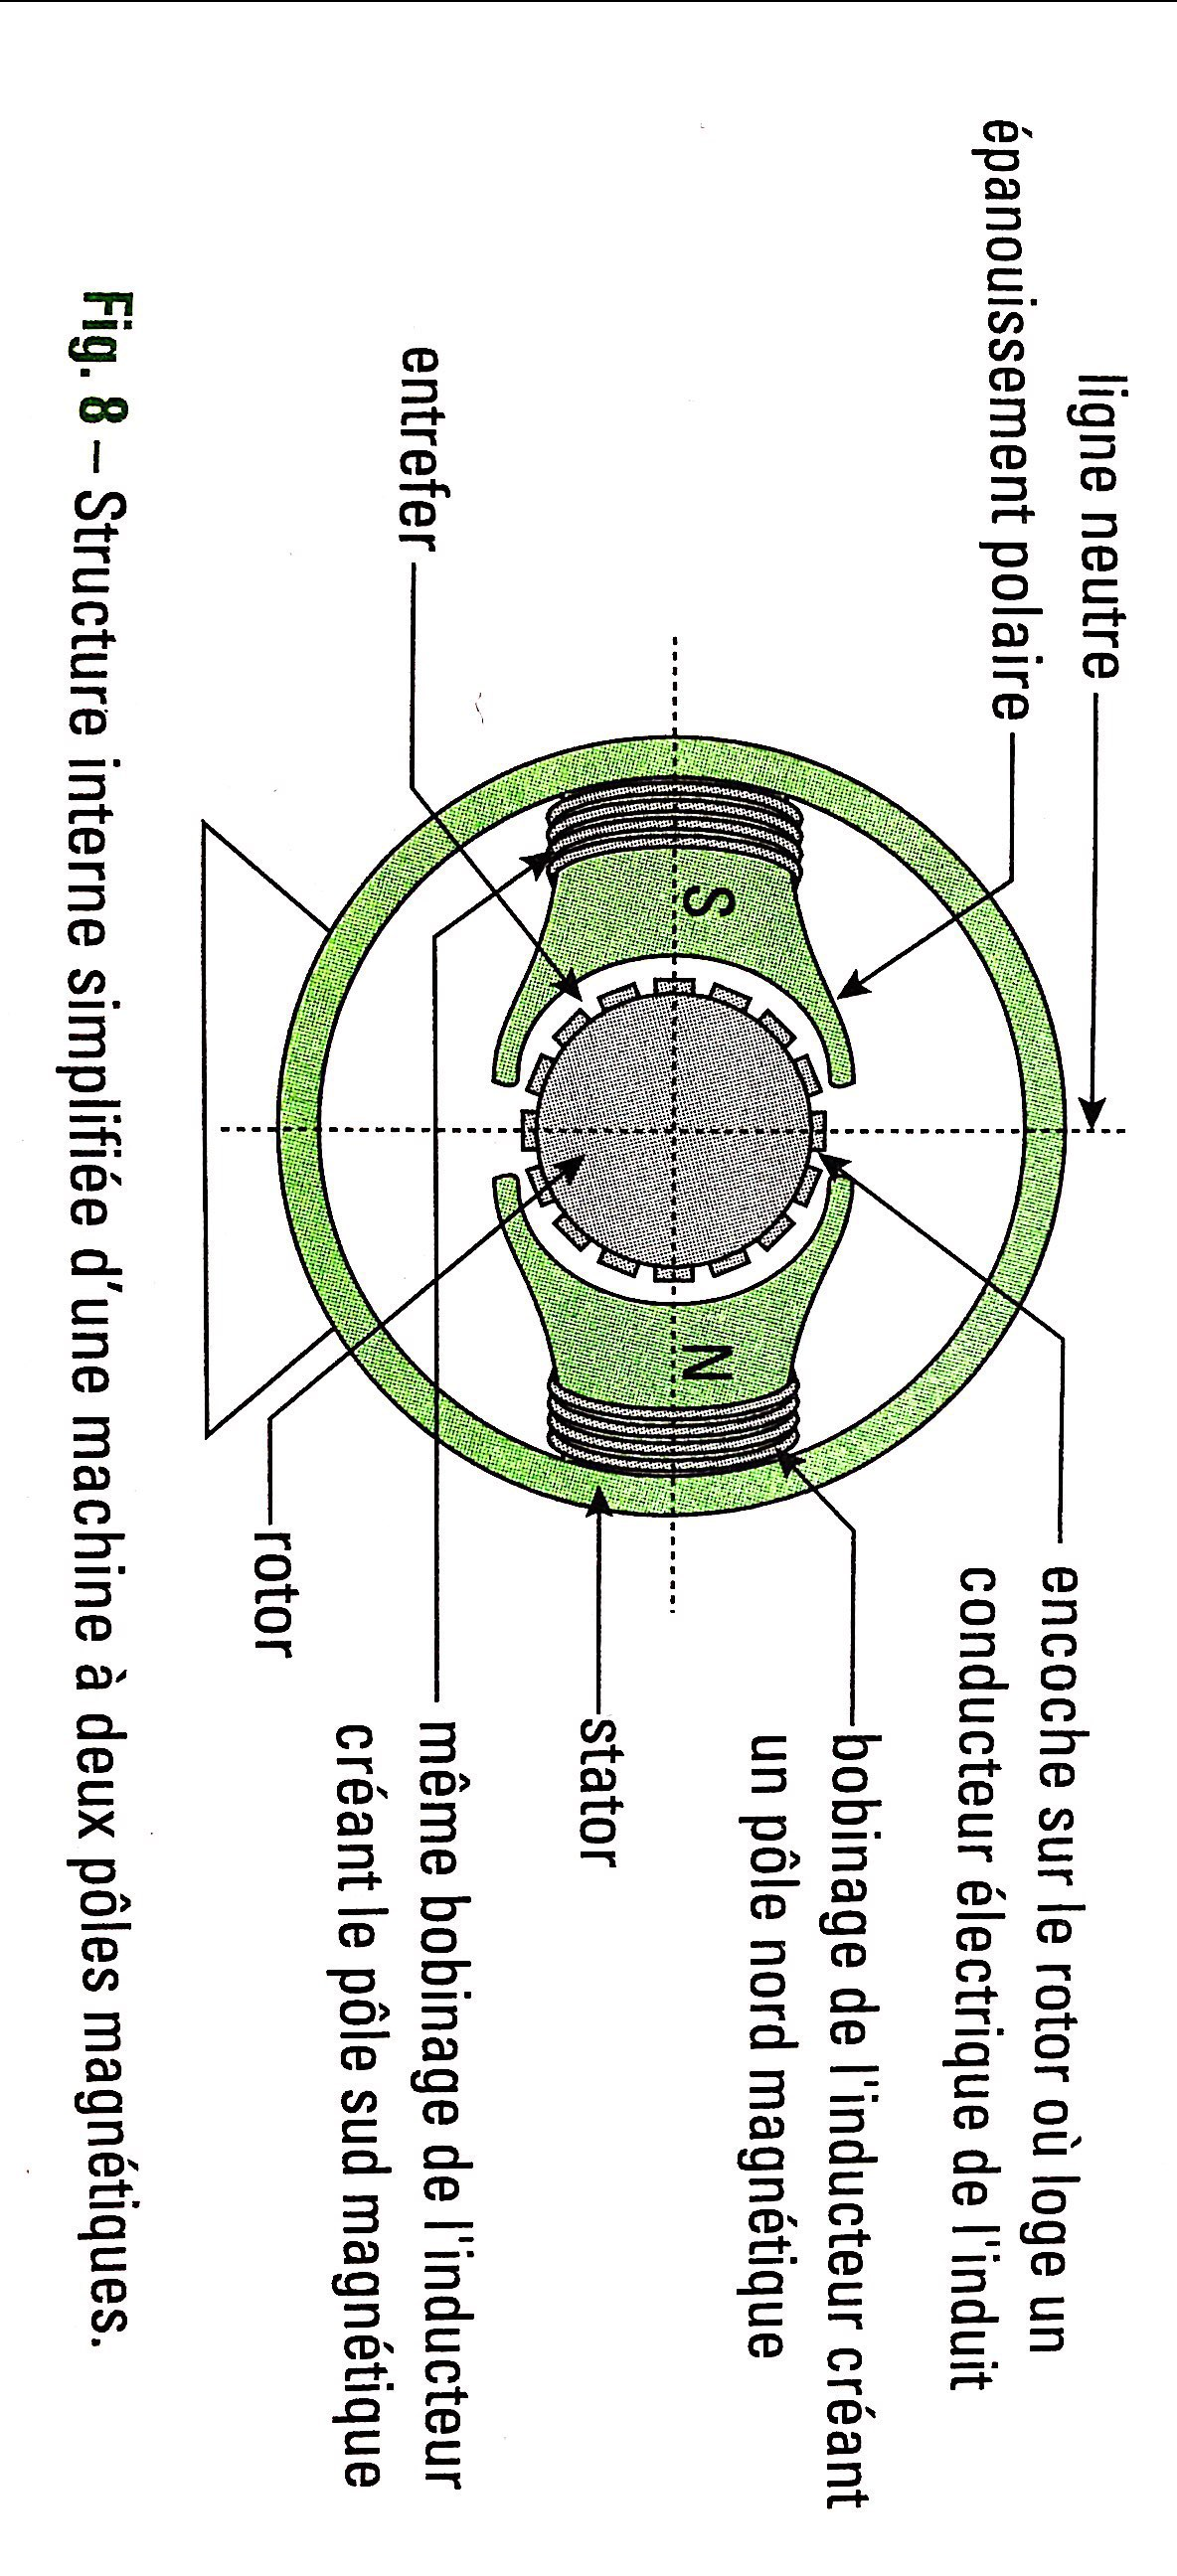
\includegraphics[width =6cm]{MoteurCC.jpg}
 %   \caption{Structure interne simplifiée d'une machine à deux pôles magnétiques}
 %   \label{fig:my_label}
%\end{figure}

\textcolor{red}{Schéma vue éclatée}


La machine à courant continue comporte deux bobinages, l'un porté par le stator et l'autre par le rotor. Le stator et le rotor, constitués d'un matériau magnétique à base de fer, sont séparés par un entrefer.\medskip

L'ensemble forme un circuit magnétique où les lignes de champ traversant l'entrefer et le rotor se referment dans le stator.\medskip

On se limite à l'étude de la machine à courant continu vérifiant les \textbf{hypothèses} suivantes :

\begin{itemize}
    \item le matériau constituant le stator et le rotor est un matériau magnétique linéaire de perméabilité magnétique relative infinie.
    \item Machine à entrefer radial et d'épaisser constante.
    \item chaque bobinage ne génère que deux pôles (nord et sud). Machine bipolaire
    
\end{itemize}


\subsubsection{Etude du circuit statorique}

Deux bobinages identiques portés par les deux cols situés de part et d'autre du rotor sont connectés en série et donc parcourus par le même courant inducteur permanent d'intensité $I_e$.\medskip

\begin{center}
    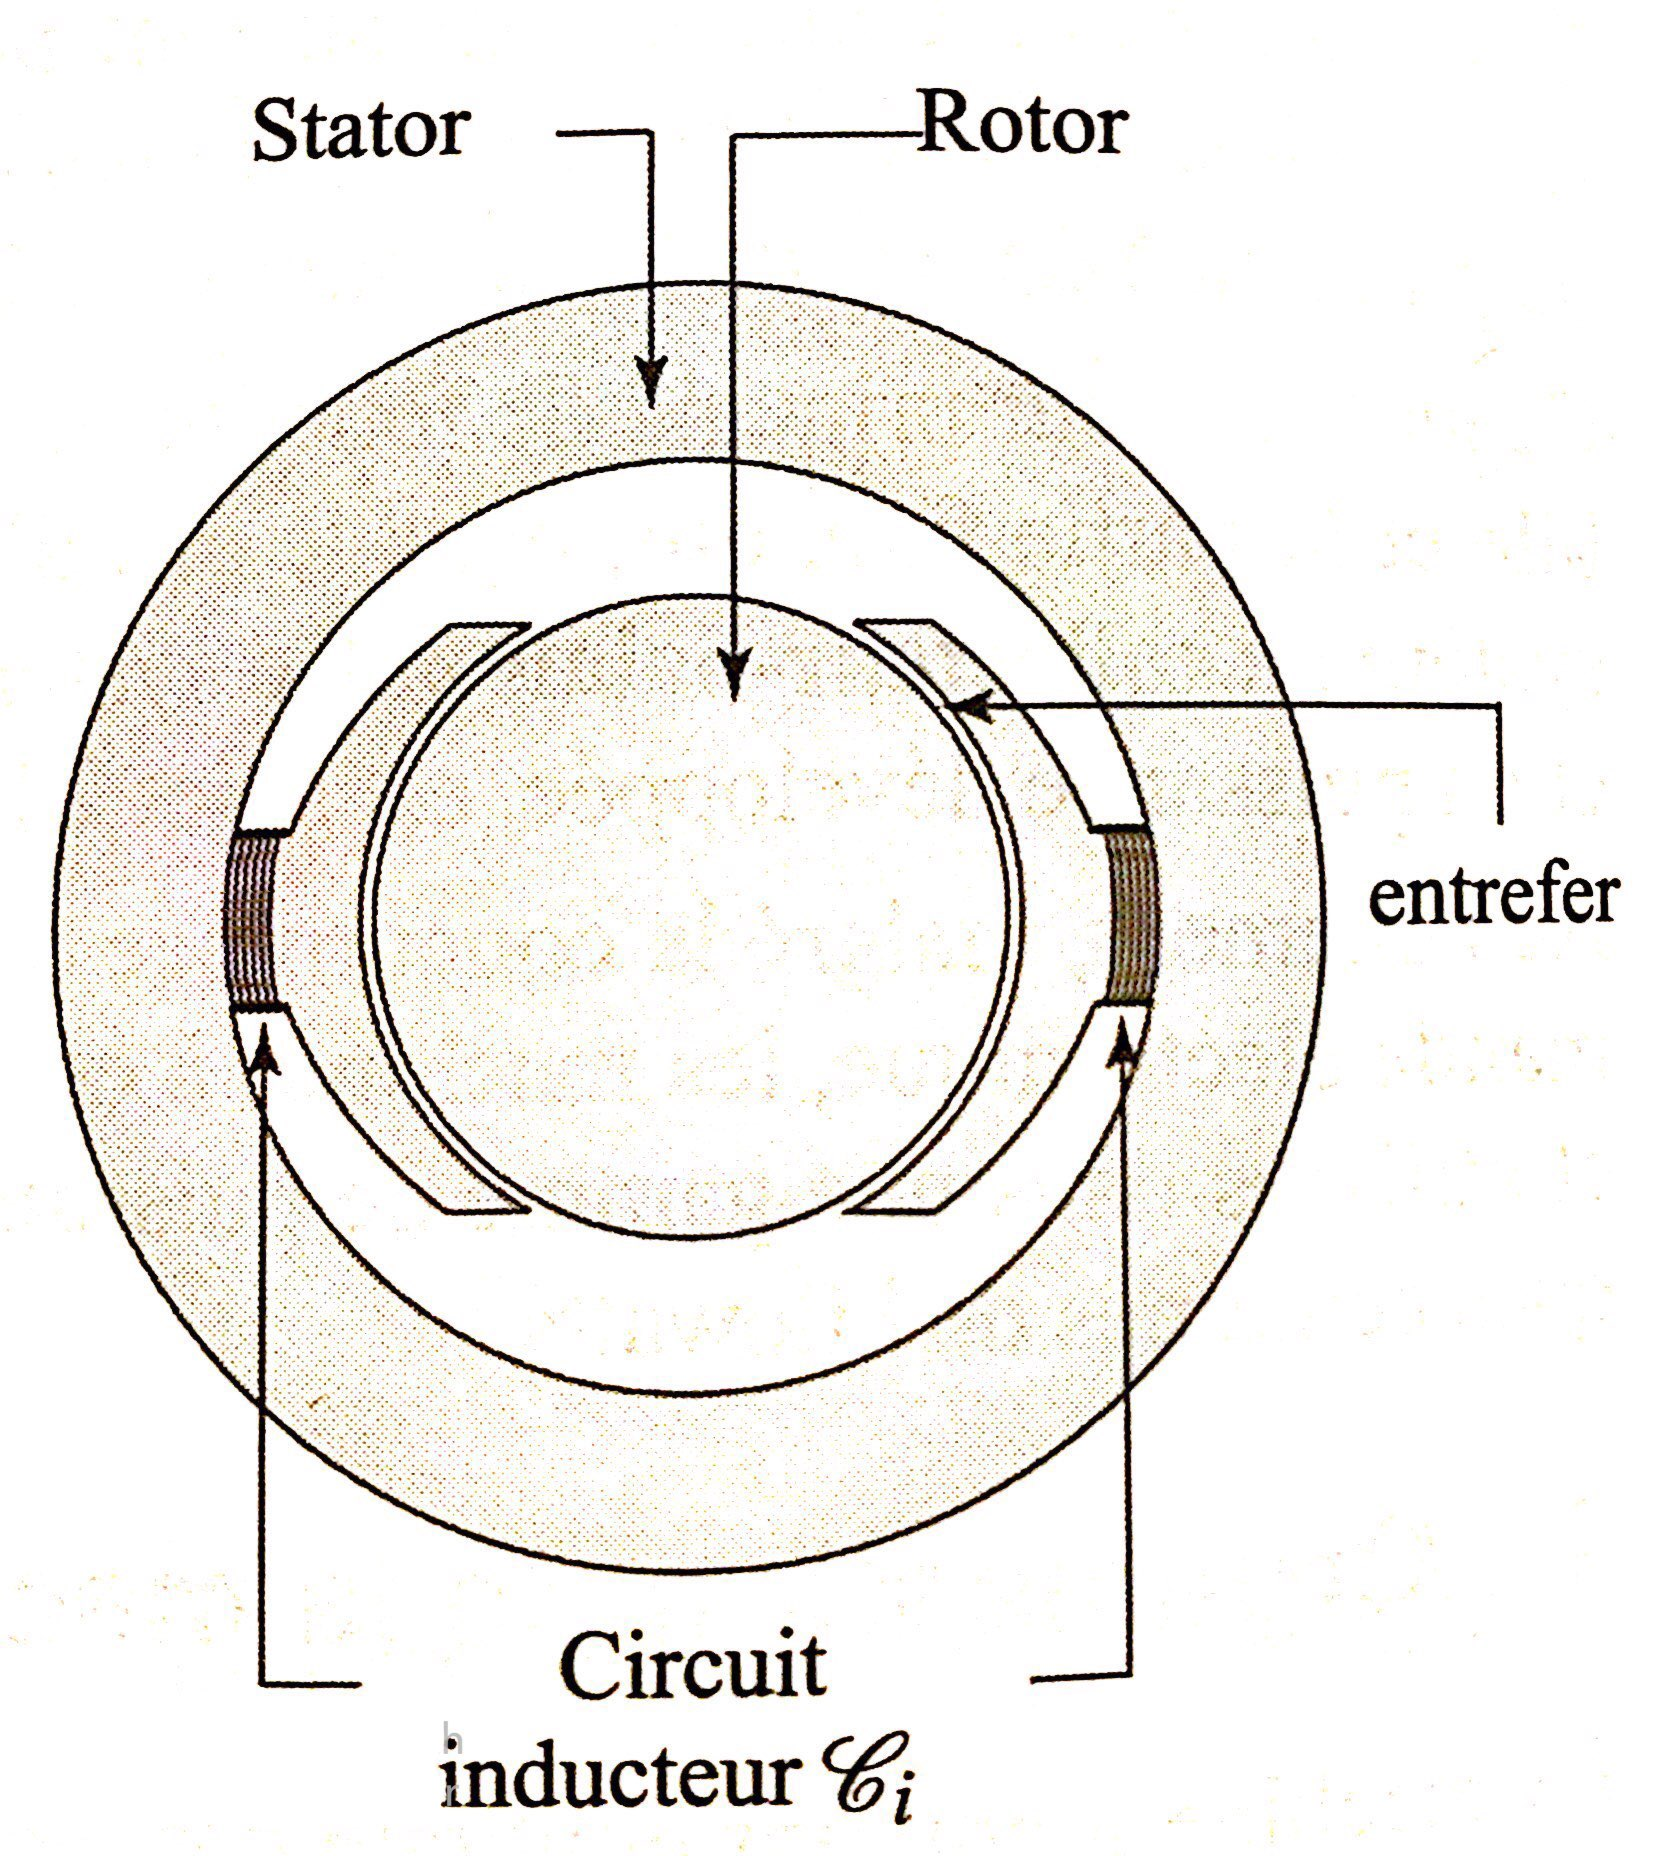
\includegraphics[scale=0.1]{stator.jpg}
\end{center}

Le champ magnétique inducteur est donc permanent. En négligeant les effets de bords, les plans orthogonaux à l'axe de rotation, tel que le plan de coupe étudié, sont des plans d'antisymétrie de la distribution de courant inducteur. Par conséquent, les lignes de champ magnétique sont contenues dans ce plan.\medskip

La simulation numérique des équations locales satisfaites par le champ magnétique permet de simuler la géométrie de ces lignes de champ.\medskip

\begin{center}
    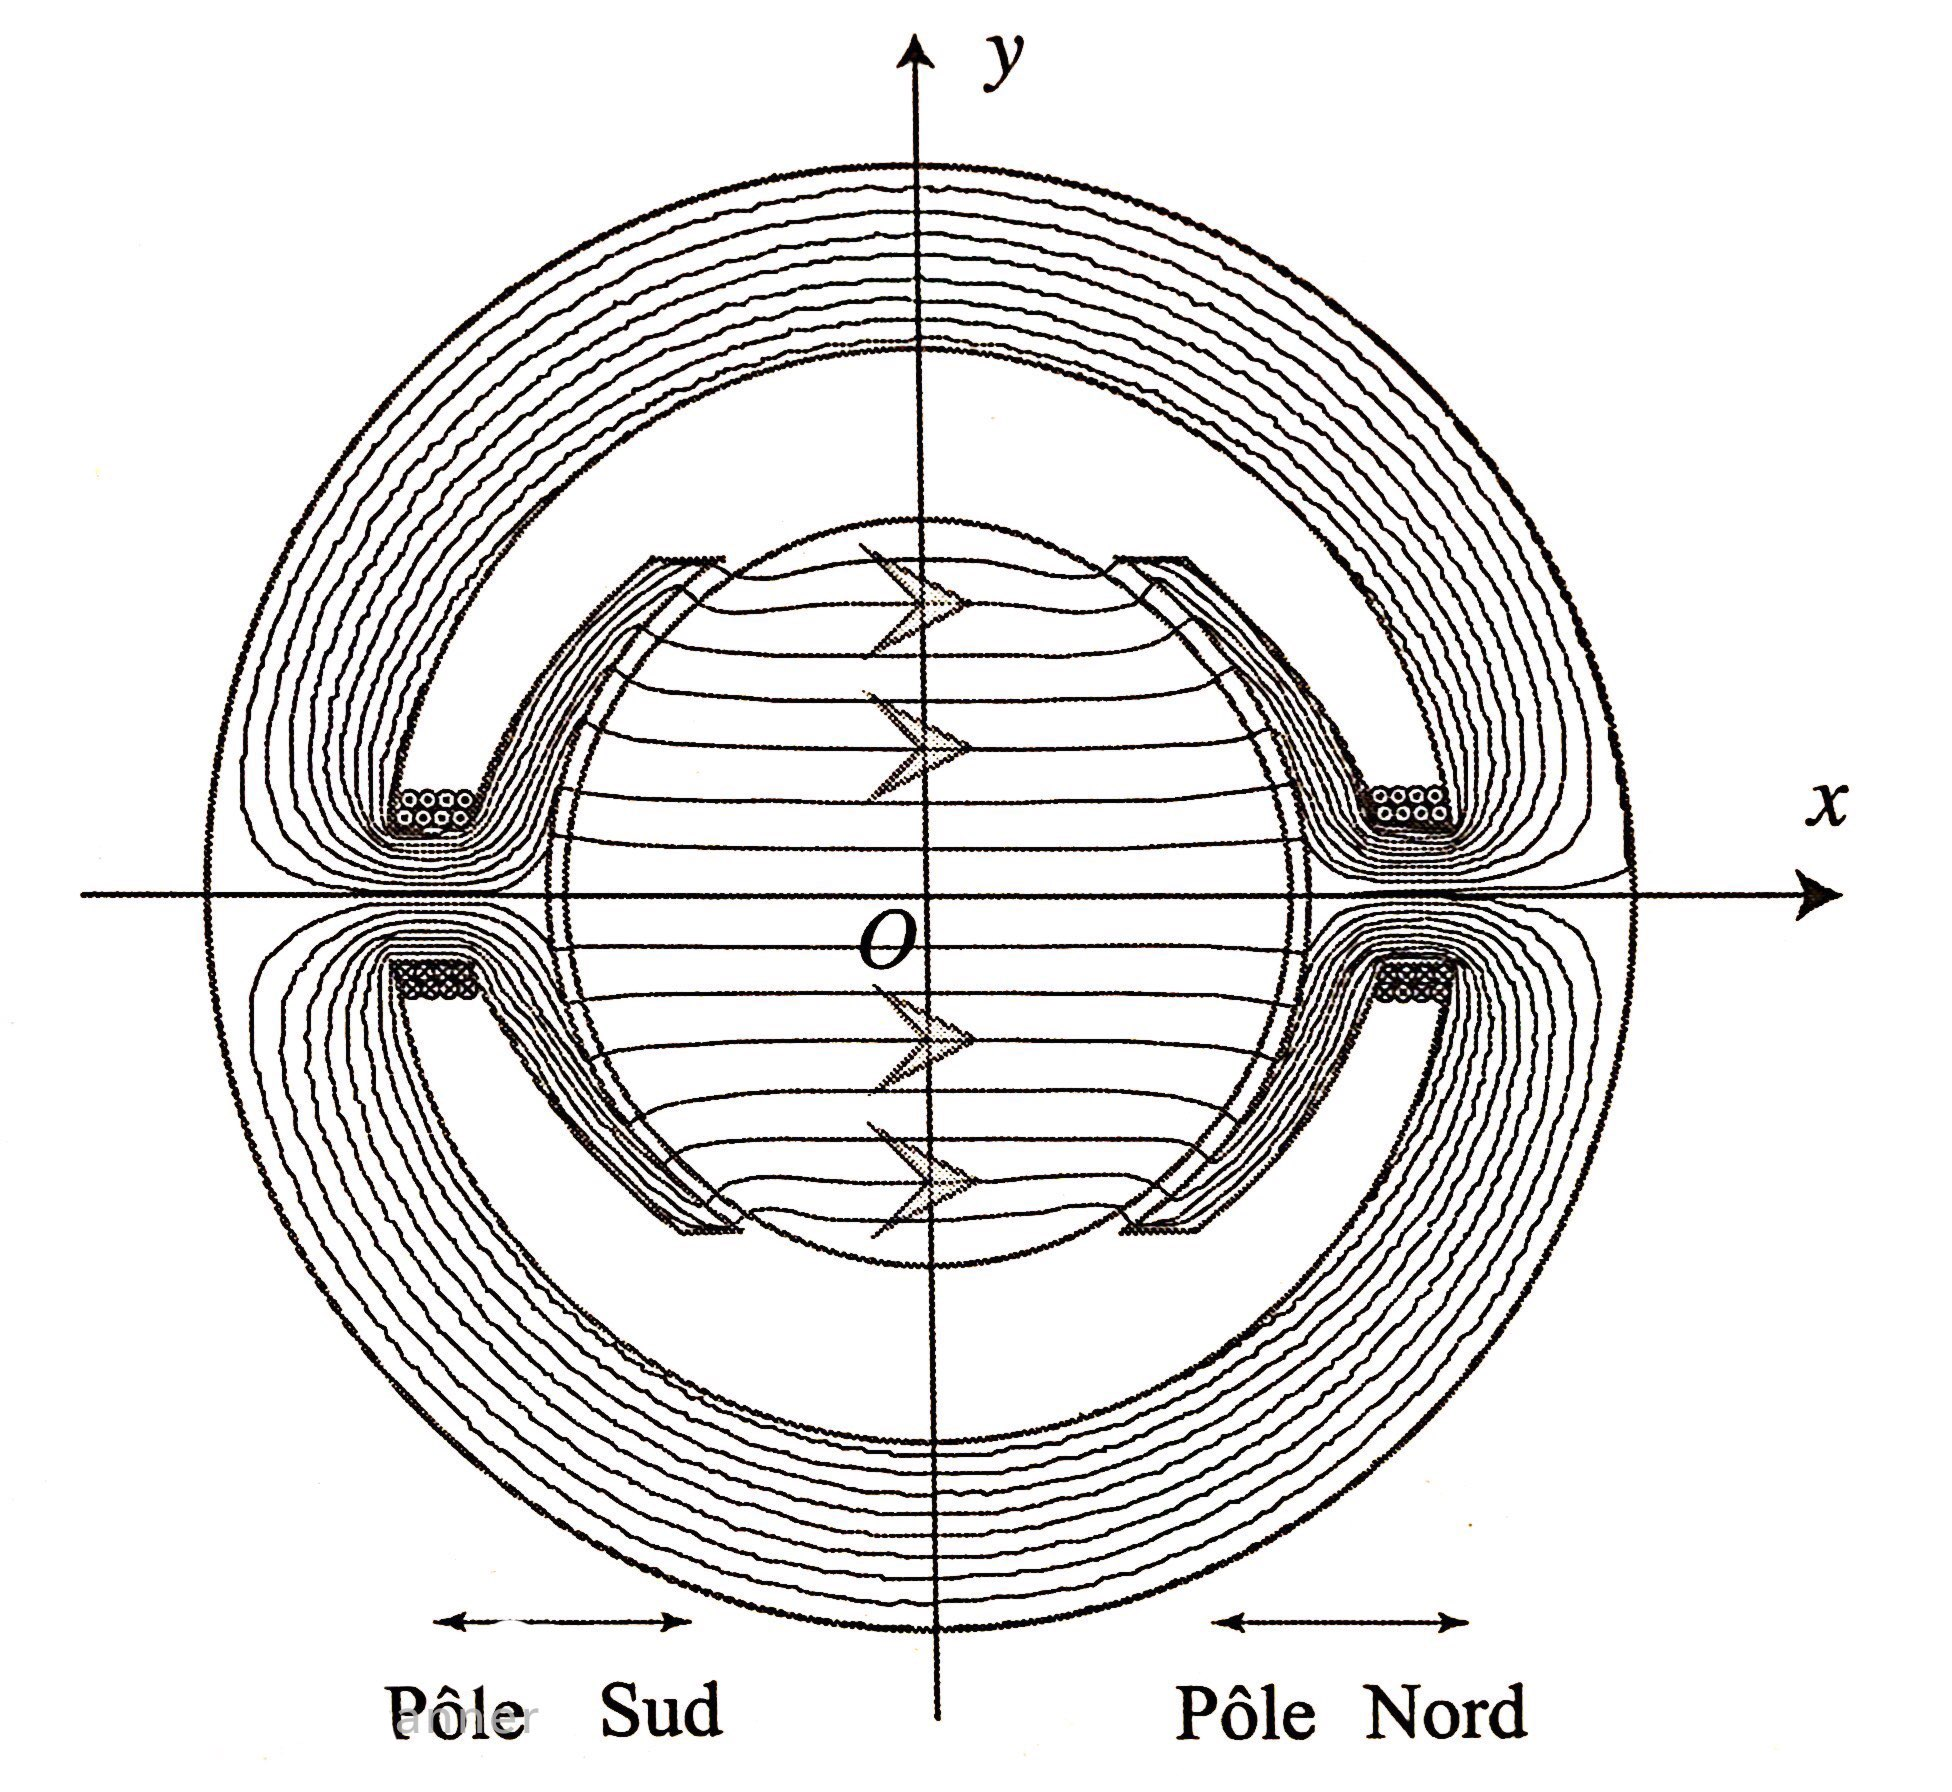
\includegraphics[scale=0.1]{LC.jpg}
\end{center}

L'entrefer étant entouré de deux cylindres en matériau de permeabilité magnétique infinie, les lignes de champ dans l'entrefer, orthogonales aux cylindres, sont radiales.\medskip

Dans la figure precedente on voit que l'axe Ox constitue l'axe polaire orienté.

\subsubsection{Etude du courant rotorique}

Le circuit rotorique nommé circuit induit, est alimenté par le courant continu $I$ qui entre dans le circuit à travers une alimentation externe. Dans la figure, nous voyons la représentation d'une spire parmi celles du circuit rotorique dont la position est repérée par l'angle $\theta$. \medskip

\begin{center}
    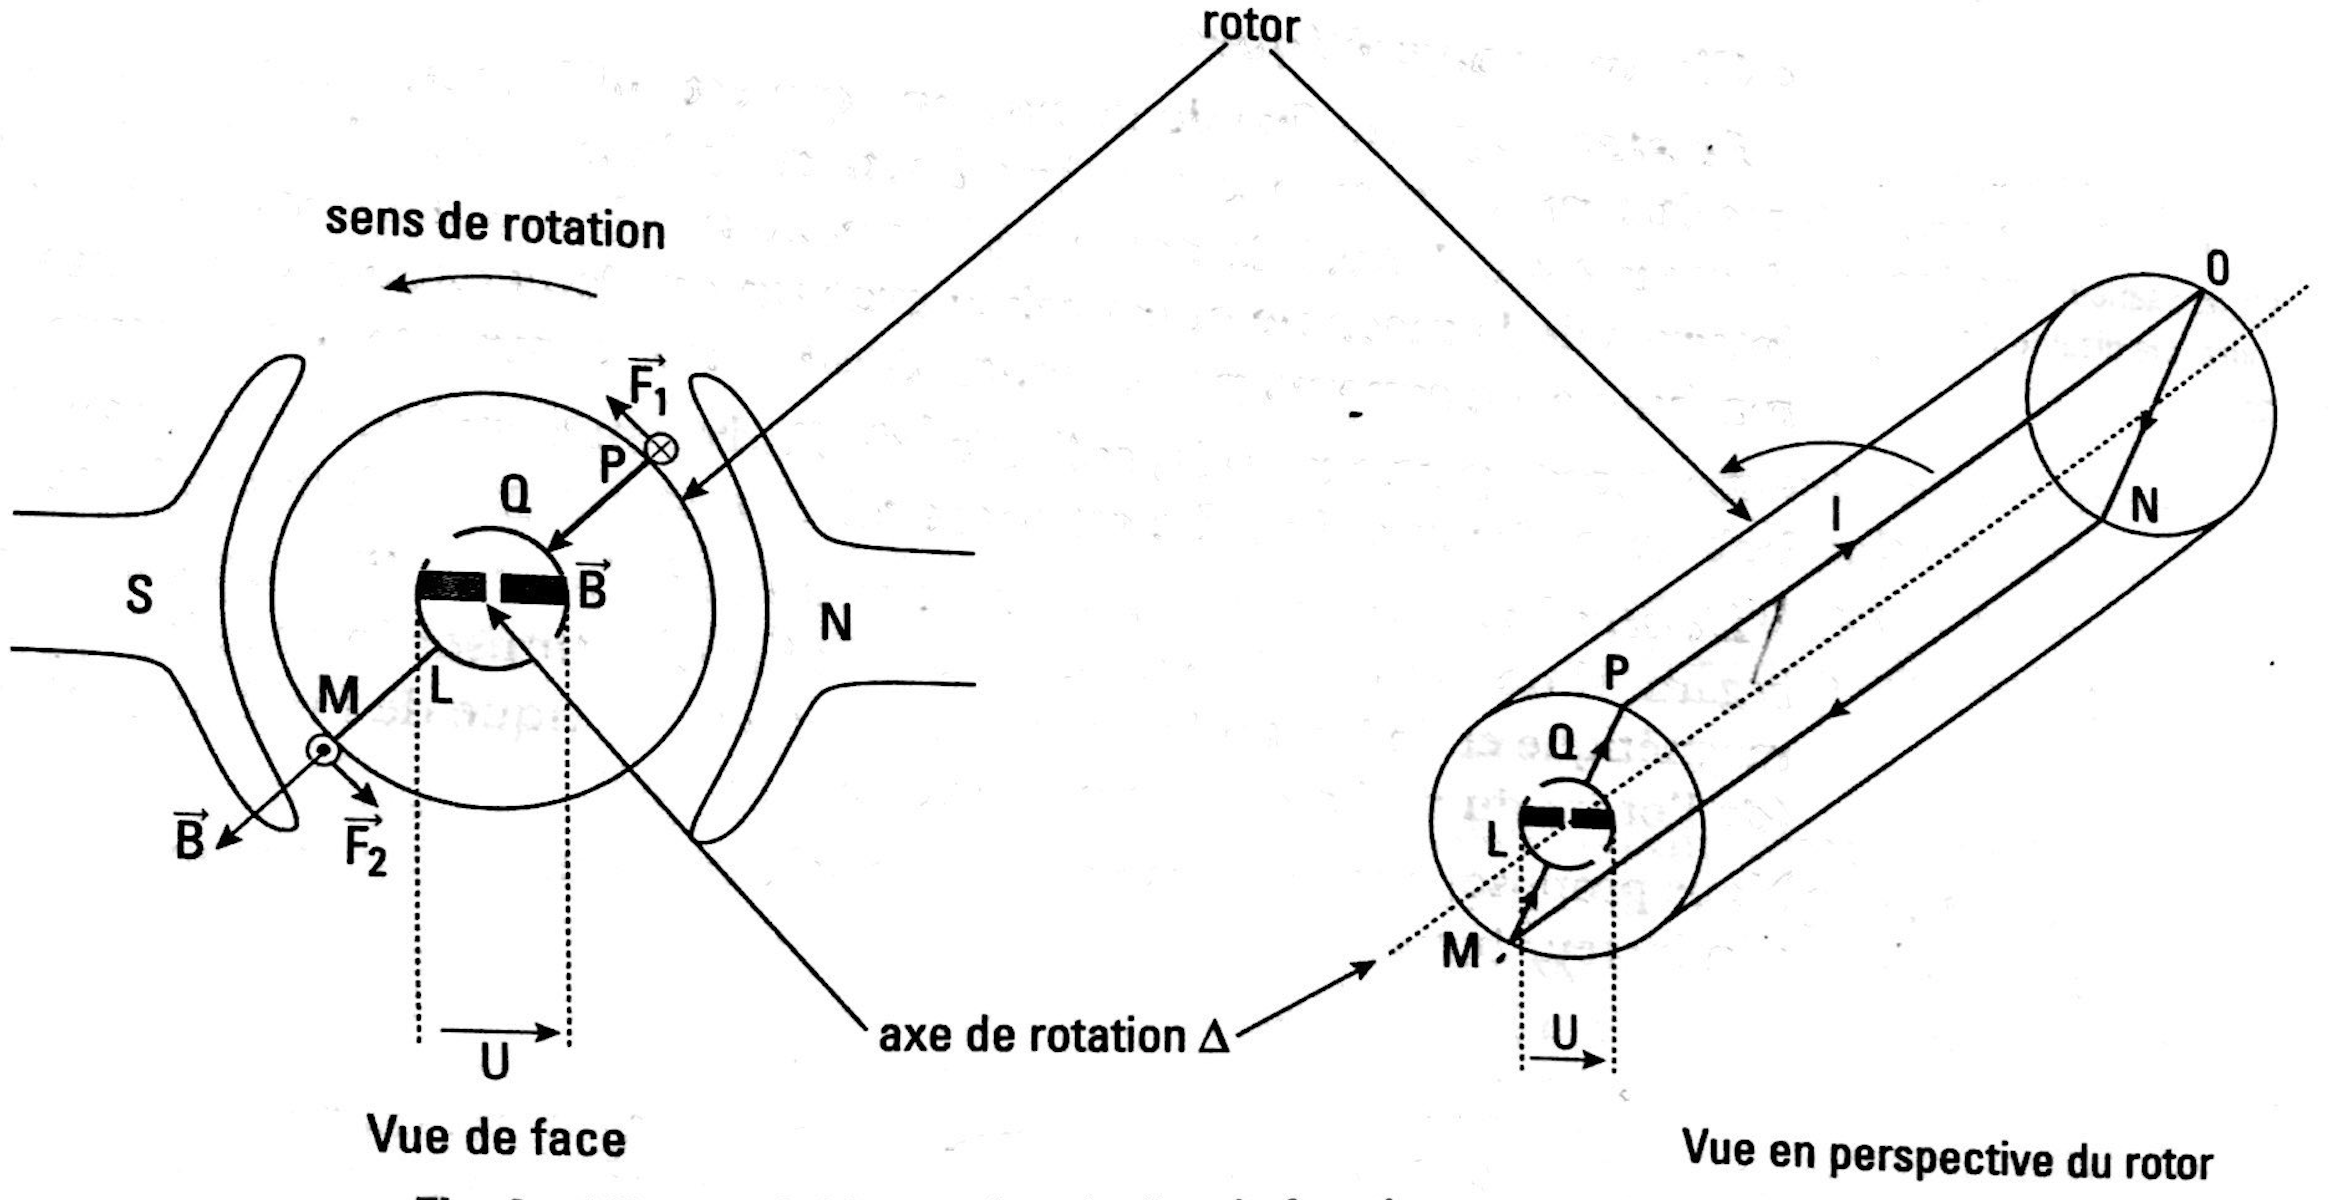
\includegraphics[scale=0.3]{mcc.png}
\end{center}


\begin{center}
    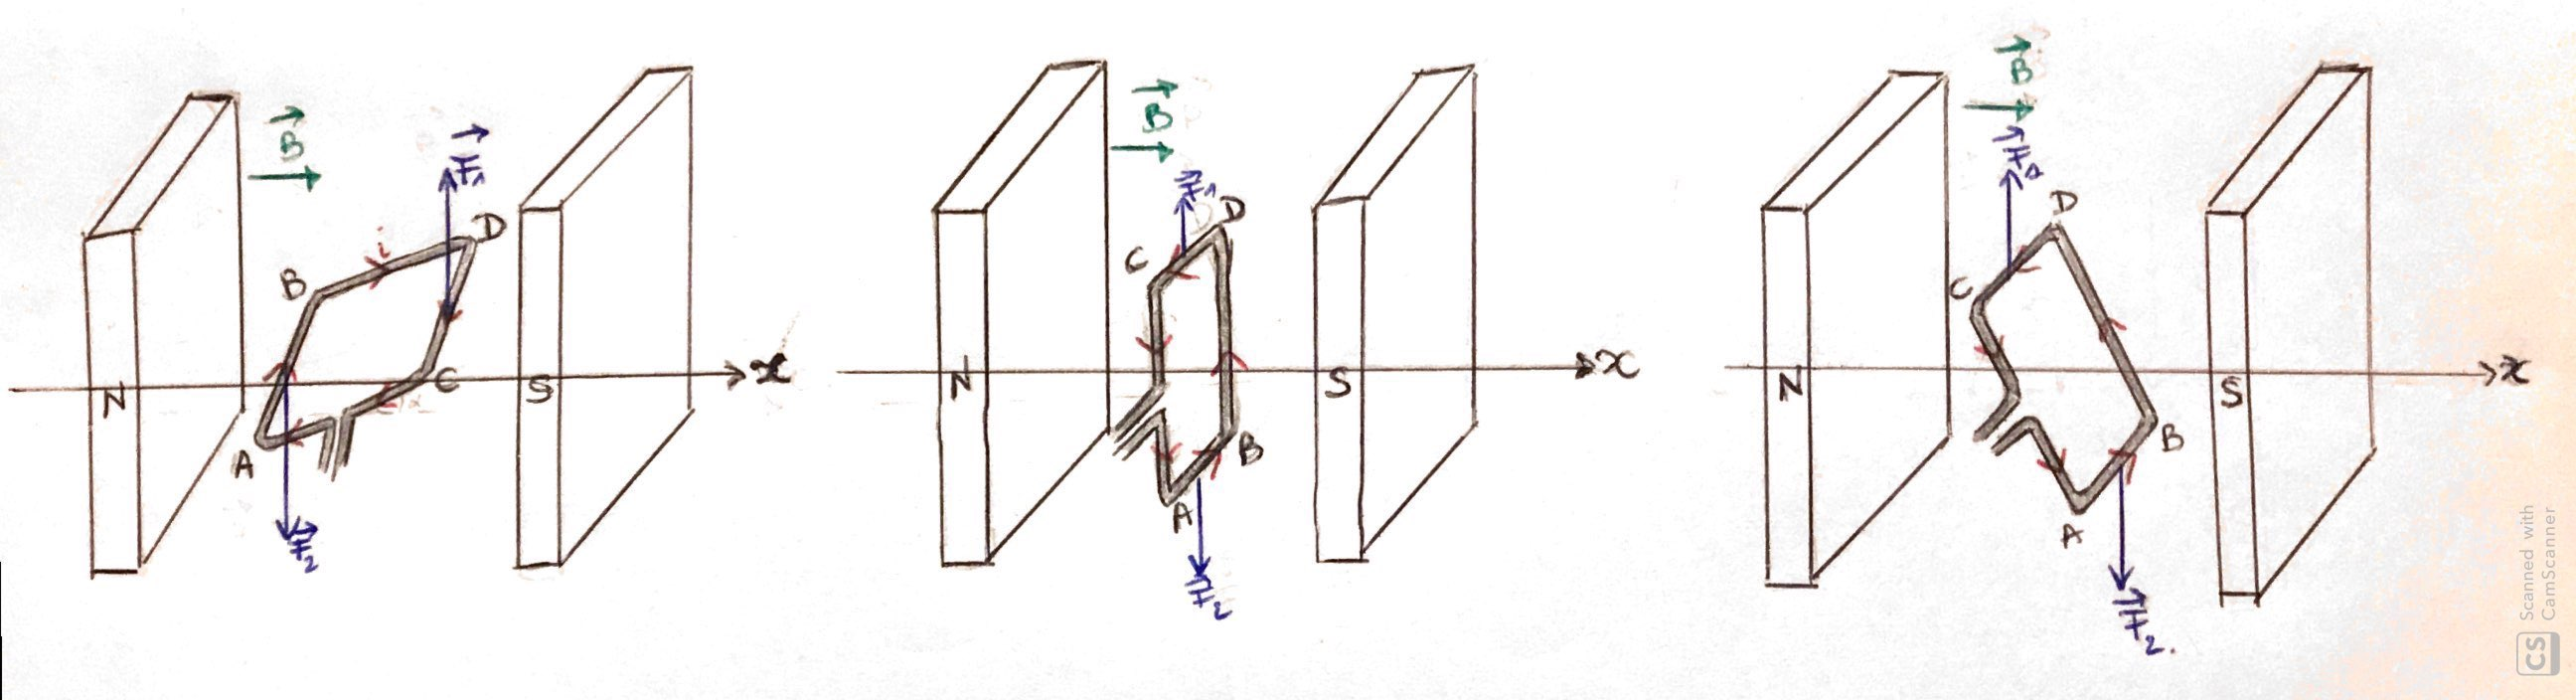
\includegraphics[scale=0.17]{spiretournemcc.jpg}
\end{center}

La connexion de cette spire au circuit d'alimentation, montre que si cette connexion restait fixe, le sens de circulation du courant pour la partie gauche de la spire située à gauche du plan $(O,y,z)$ s'inverserait en fonction de $\theta$ à la période de $\pi$. \medskip

Ce sont les forces de Laplace qui sont responsables du mouvement mécanique du rotor, comme dans le cas des rails de Laplace. Les brins $BD$ et $AC$ ne participent pas au mouvement de rotation car... Les conducteurs $AB$ et $CD$ sont soumis à une force de Laplace dont la résultante est nulle car ils sont de même longueurs et parcourus par des courants de même intensité et de sens opposé :

\begin{equation}
    \vec{F_1} + \vec{F_2} = \vec{0}
\end{equation}

où

\begin{equation}
    \vec{F_1} = I\vec{l} \land \vec{B} = IRB \vec{u_\theta} = -\vec{F_2}
\end{equation}

Le torseur des actions mécaniques se réduit donc à un couple des forces électromagnétiques.\medskip

On note $l$ la longueur des conducteurs $AB$ et $BC$, ils sont traversés par un courant $I$, tout comme la spire dont la longueur est égale au rayon du rotor $R$. Le couple résultant exercé sur la spire ABCD dans le repère cylindrique de base (O, $\vec{u}_r, \vec{u}_{\theta},\vec{u}_z$), avec O sur l'axe de rotation du rotor, est :

\begin{equation}
    \vec{\Gamma} = R\vec{u_r} \land \vec{F_1} + (-R\vec{u_r} \land \vec{F_2})
\end{equation}

On obtient :

\begin{equation}
    \vec{\Gamma} = 2RIlB \vec{u_z}
\end{equation}

Le module $C$ de ce couple est appelé \textbf{moment du couple électromagnétique}, ou plus simplement \textbf{couple électromagnétique}, tel que : $C = 2RIlB$. \medskip


Il est possible de transformer cette dernière écriture en remarquant que le terme $2Rl$ est homogène à une surface et $2RlB$ à un flux magnétique que nous noterons par la suite $\Phi_0$.

On peut alors écrire que le \textbf{Couple de Laplace} qui s'exerce sur la spire $ABCD$ s'exprime par :

\begin{equation}
    C = \Phi_0 I
\end{equation}

Le flux s'exprime en $V.s$ ou en weber ($Wb$), le moment du couple en $N.m$ et l'intensité de courant en $A$.\medskip

Nous constatons que lorque $\Phi_0$ est constant, le couple électromagnétique C est directement proportionnel à l'intensité électrique $I$. \medskip

En pratique c'est bien le cas car le circuit inducteur travaille à flux constant. Par conséquent, la grandeur qui contrôle le couple est l'intensité électrique I qui traverse le circuit induit.\medskip

D'autre part, il est important de comprendre qu'en régime permanent, c'est la charge mécanique du moteur qui imposera le couple résistant et, par conséquent, la valeur de C (aux éventuelles pertes près). Le débit de courant dans l'induit du moteur est donc l'image de cette charge entraînée par le moteur.


\subsubsection{F.e.m d'induction E}

La loi de conservation de la puissance électromagnétique $P_m + P_e =0$ donne, en tenant compte du signe des grandeurs en convention récepteur :
\begin{equation}
    P_m = P_e
\end{equation}
En notant $\Omega$ la vitesse angulaire de rotation du rotor, nous avons :
\begin{eqnarray}
    P_m = \vec{\Gamma}\vec{\Omega}= C \Omega = \Phi_0 I \Omega\hspace{1cm}\mathrm{et}\hspace{1cm}
    P_e = EI
\end{eqnarray}
On obtient alors que $E= \Phi_0 \Omega$. \medskip

En régime établi, on peut en première approximation négliger la chute de tension résistive RI dans l'induit, ce qui permet d'écrire que $U \approx \Phi_0 \Omega$ car les conducteurs de l'induit sont choisis peu résistants afin de limiter les pertes par effet Joule. On peut alors piloter la vitesse de rotation du moteur par l'intermédiaire de la valeur de la tension U.


\begin{center}
    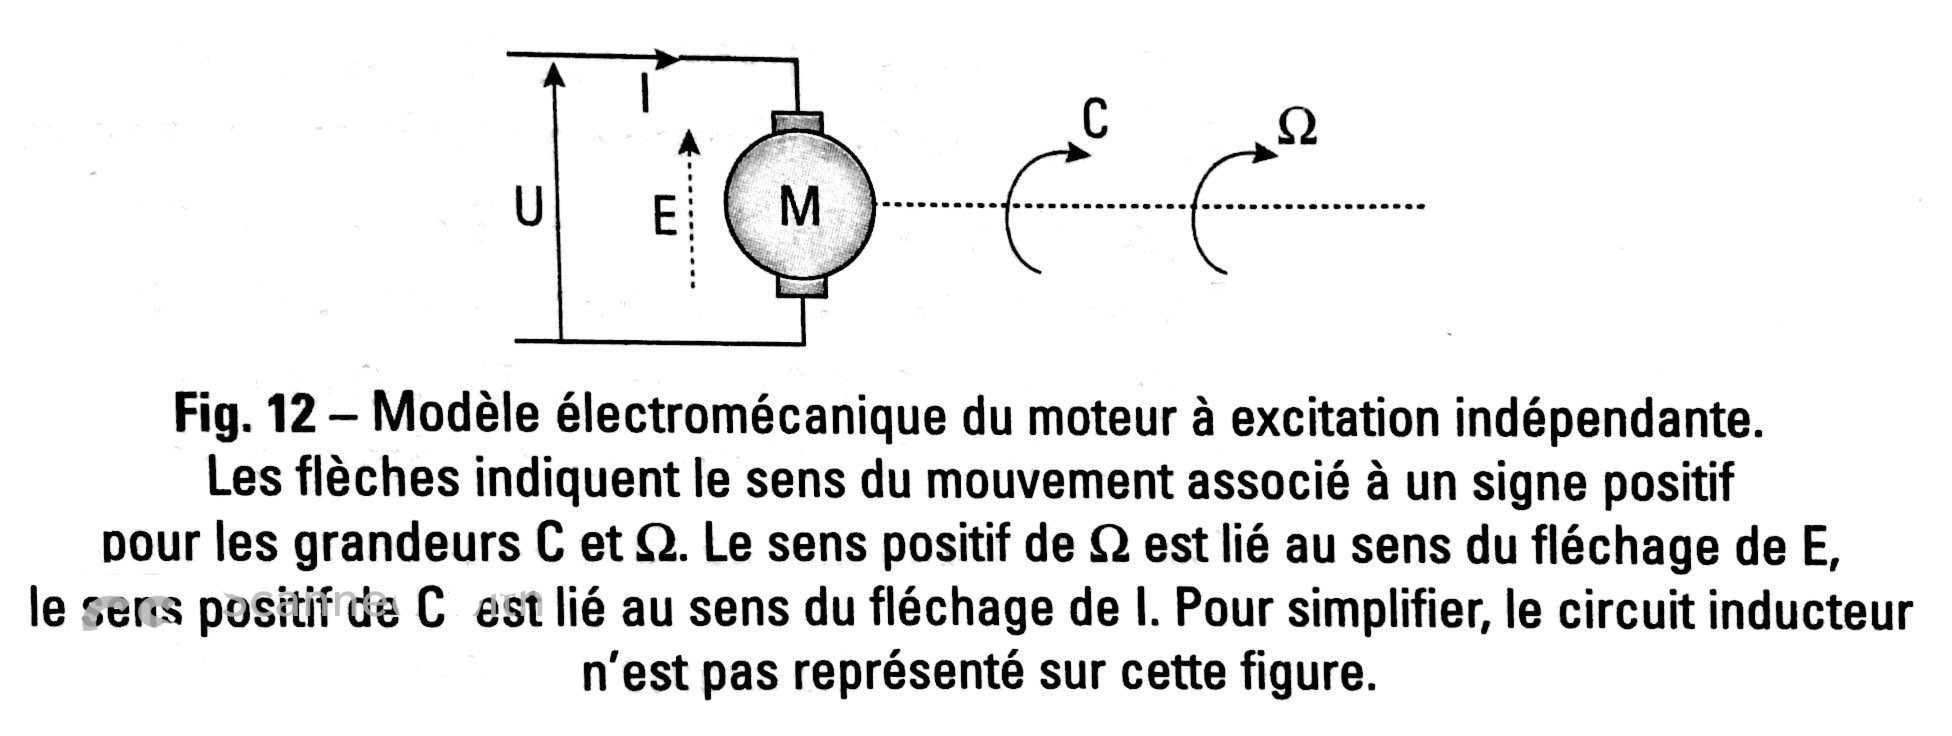
\includegraphics[scale=0.14]{convention.jpg}
\end{center}


\subsubsection{Modes de fonctionnement}

En conservant toujours la même convention pour l'orientation de la f.e.m induite E, on a  :

\begin{itemize}
    \item $E > 0$ et $I>0$ (convention récepteur). Ainsi la machine fonctionne en moteur : $EI>0$, elle reçoit de la puissance électrique et fournit de la puissance mécanique.
    \item Au contraire, la machine fonctionne en mode génératrice lorsque $EI<0$ (convention recepteur), la machine reçoit de la puissance mécanique et fournit de la puissance électrique.
\end{itemize}

Nous pouvons détailler cette propriété en envisageant différents cas selon le signe de $\Omega$. Ce sont les quatre quadrants de la machine à courant continu : \textcolor{red}{mettre moteur ou générateur sur l'image}


\begin{center}
    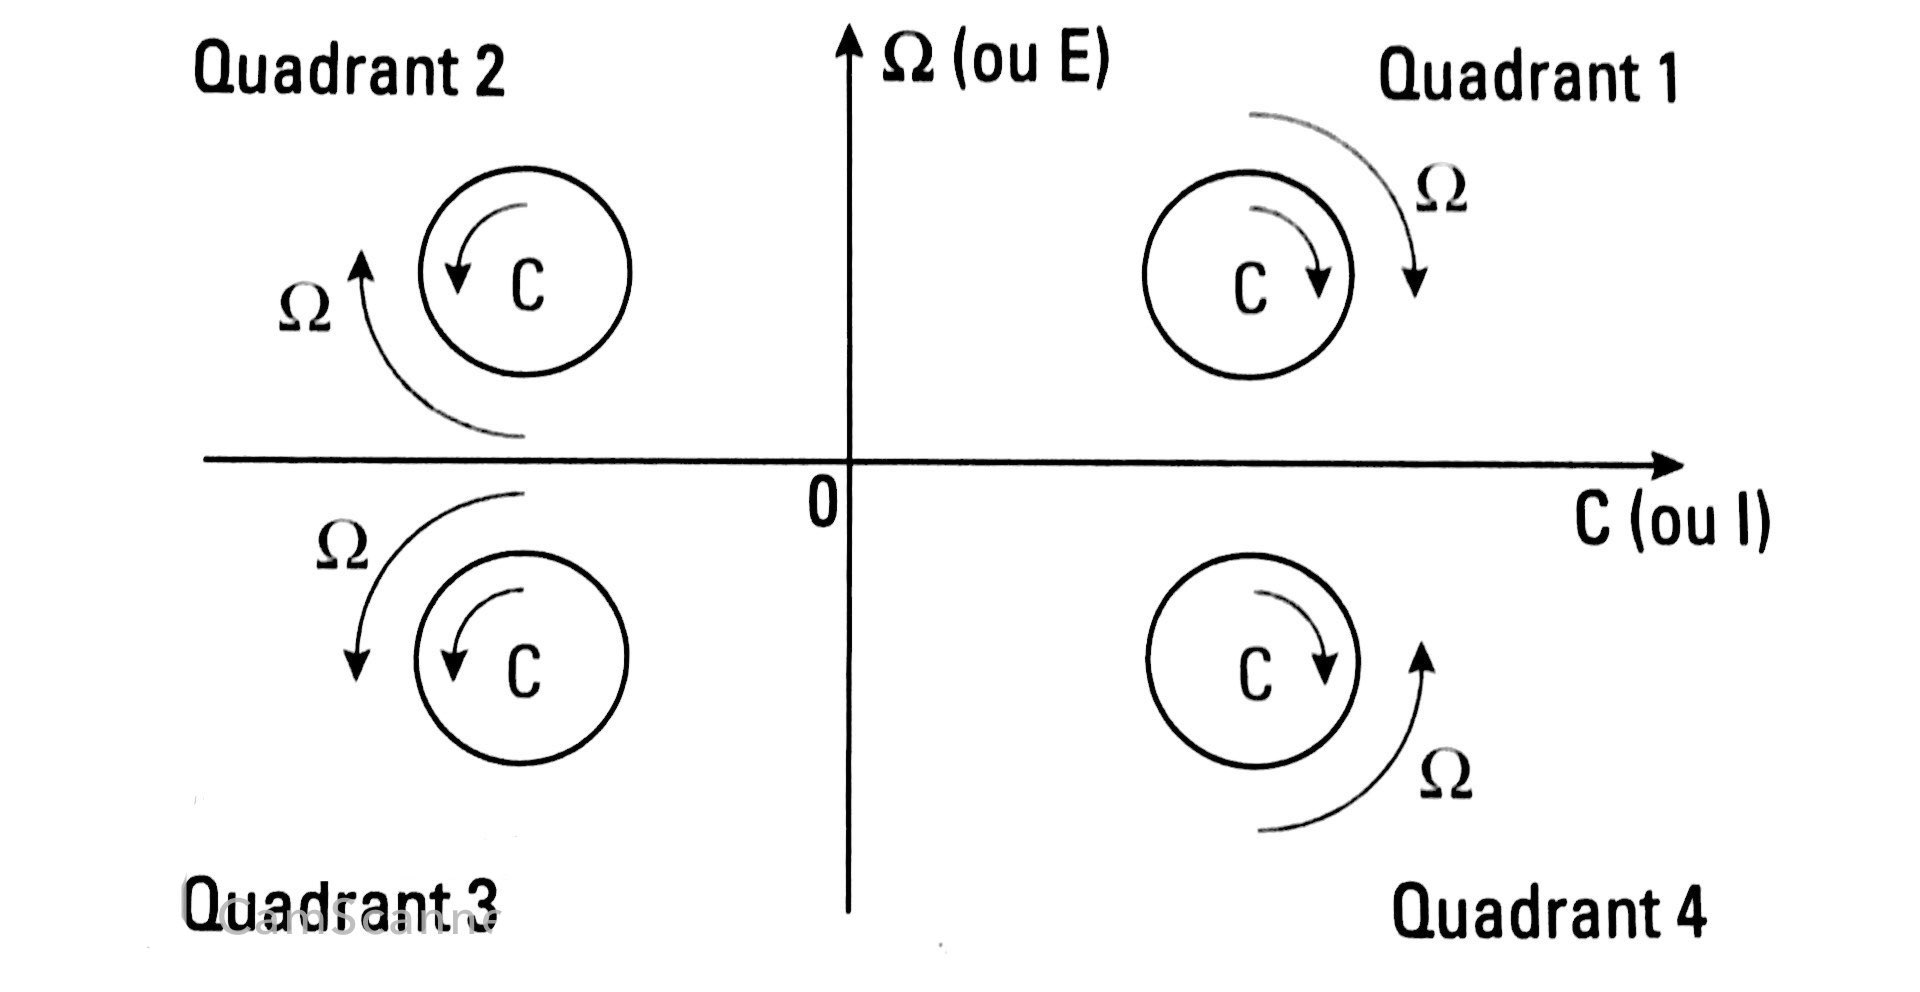
\includegraphics[scale=0.18]{quadrants.jpg}
\end{center}


\begin{itemize}
    \item Quadrant 1: $EI>0$ avec $E>0$ (donc $\Omega >0$) et $I>0$. Moteur qui tourne dans le sens positif choisi.
    \item Quadrant 2: $EI<0$ avec $E>0$ et $I<0$. La machine fonctionne en génératrice et tourne dans le sens positif.
    \item Quadrant 3: $EI>0$ avec $E<0$ et $I<0$. La machine fonctionne en moteur et tourne dans le sens négatif.
    \item Quadrant 4: $EI<0$ avec $E<0$ et $I>0$. La machine fonctionne en génératrice et tourne dans le sens négatif.
\end{itemize}

\subsubsection{Modèle électromécanique équivalent}

\begin{itemize}
    \item \textbf{Comportement en régime établi}. 
    \begin{equation}
        U = E + RI
    \end{equation}
    \item \textbf{Comportement en régime dynamique ou transitoire}. 
    \begin{equation}
        U(t) = E(t) + RI(t) + L \frac{dI (t)}{dt}
    \end{equation}
\end{itemize}


\begin{tabular}{cc}
   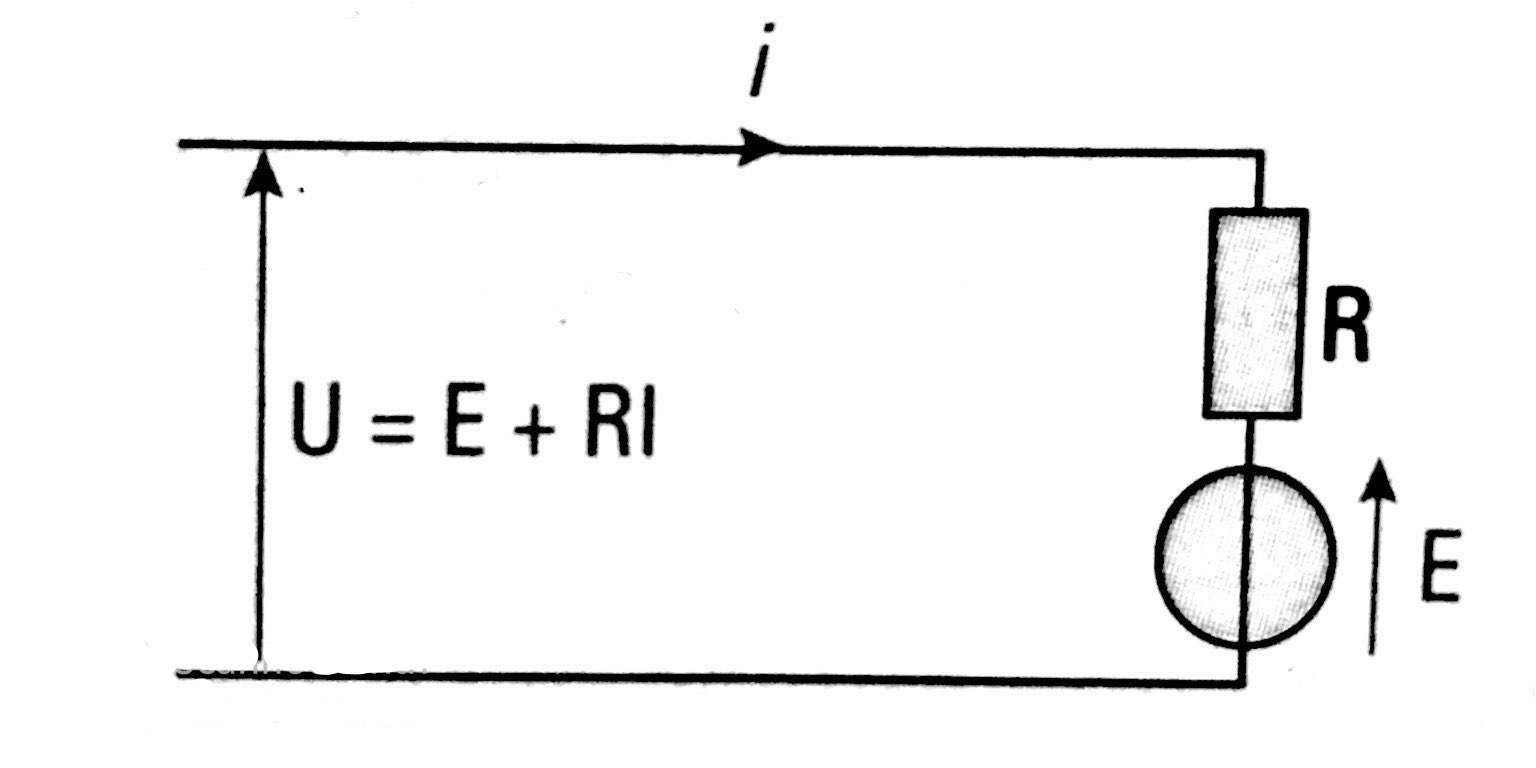
\includegraphics[scale=0.11]{etabliMCC.jpg} &
   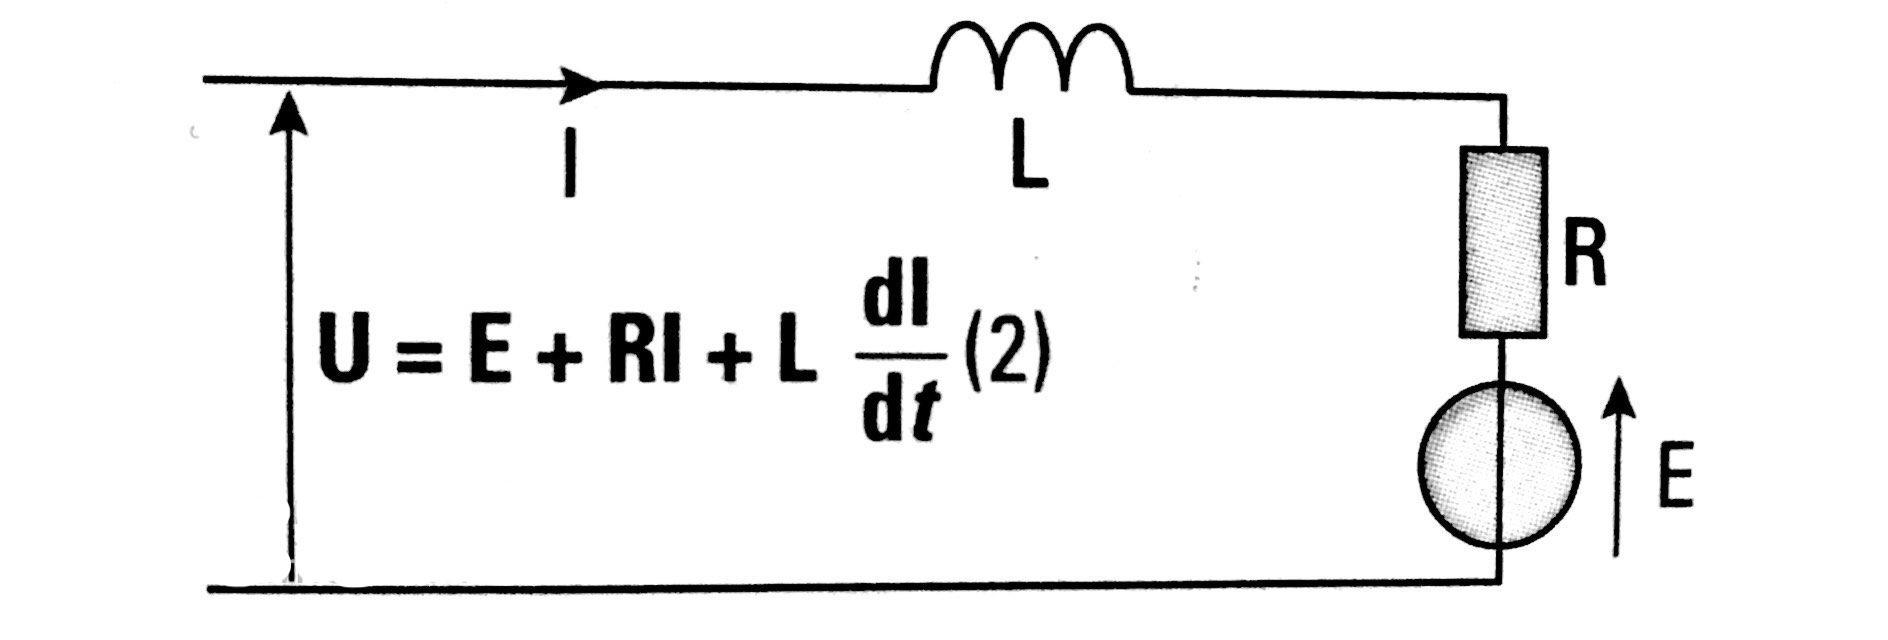
\includegraphics[scale=0.11]{dynamMCC.jpg} \\
\end{tabular}



\subsubsection{Démarrage de la machine}

Par définition lorsqu'une machine démarre, sa vitesse initiale est nulle. Le courant de l'induit n'est donc limité que par la résistance des bobinages qui le constituent :

\begin{equation}
    U = E + RI = RI (E=\Phi_0\Omega=0)
\end{equation}

Par conséquent, le courant circulant dans l'induit est, dans ce cas, élévé puisqu'en pratique la résistance $R$ est faible. Il est donc nécessaire de démarrer la machine sous tension réduite afin de ne pas dépasser le courant maximal admissible par l'induit. La solution industrielle classique consiste à augmenter progressivement la tension de l'induit $U$ par variateur de vitesse. Ceci peut être réalisé grâce au \textbf{montage hacheur}.

\subsubsection{Emballement de la machine à excitation indépendante}

\begin{equation}
    U = E + RI
\end{equation}
avec $E=\Phi_0 \Omega$. On obtient :
\begin{equation}
    \Omega = \frac{U - RI}{\Phi_0}
\end{equation}

Supposons que cette machine fonctionne à vide (son axe n'est soumis à aucun couple de charge résistant). Le flux $\Phi_0$ est créé par le circuit inducteur. Si ce dernier est bobiné, il est alors alimenté par un circuit extérieur qui lui fournit un courant d'intensité $I_e$. Si au cours du fonctionnement, le courant inducteur $I_e$ est supprimé (suppression de l'alimentation de l'inducteur), alors $\Phi_0$ s'annule et la vitesse tend mathématiquement vers l'infini. En pratique, le surcroît d'énergie cinétique peut se traduire par un emballement de la machine. Il faut donc veiller à ne jamais couper l'alimentation du circuit inducteur d'une machine à excitation indépendante. 

\subsubsection{Bilan de puissance du moteur à courant continu}

La machine absorbe la puissance électrique $UI$ absorbée à l'induit, ajoutée à celle éventuellement absorbée par l'inducteur $U_e I_e$, lorsque celui-ci est bobiné. La puissance $U_e I_e$ est entièrement dissipée par effet Joule, donc $U_e I_e = R_e I_e^2$.\\
La puissance absorbée à l'induit s'écrit $P = (E + RI)I = EI + RI^2$. Ceci montre qu'une puissance $RI^2$ est aussi perdue par effet Joule au niveau de l'induit du moteur. La puissance $P_e$ alors disponible est alors $EI$, qui est aussi égale à $C\Omega$. Cette puissance est usuellement appelée puissance électromagnétique.\medskip

Pour un bilan complet, il faut tenir compte des éventuelles pertes mécaniques (frottements sur roulements par exemple) et magnétiques au rotor (par hystérésis ou courants de Foucault). Ces pertes sont appelées pertes collectives et notées $P_c$. La puissance mécanique réellement disponible est appelée puissance utile, elle est de nature mécanique et donc il est possible de définir un moment de couple utile $C_u$ tel que $P_u = C_u \Omega$.\medskip

Le rendement d'un moteur à courant continu est le rapport de la puissance mécanique utile divisée par la puissance électrique totale absorbée : 
\begin{equation}
    \eta = \frac{P_u}{P_a} = \frac{P_u}{P_u + P_c + RI^2 + R_e I_e^2}
\end{equation}

\medskip

\begin{center}
    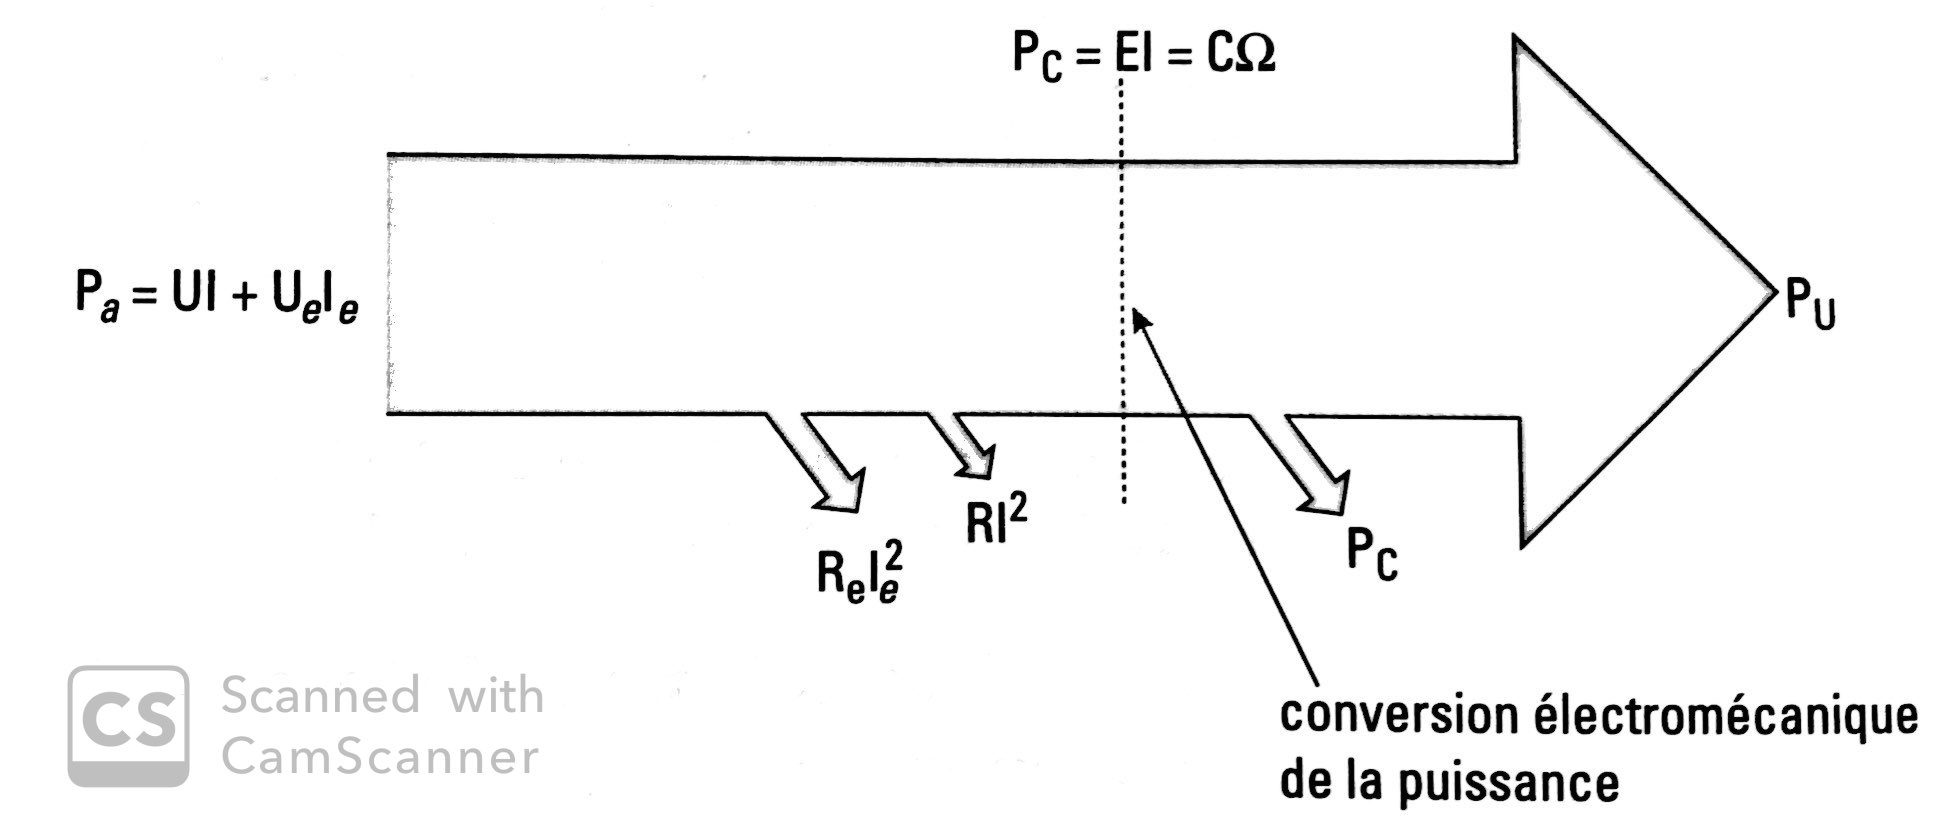
\includegraphics[scale=0.18]{puissancemoteur.jpg}
\end{center}


Dans le cas de fonctionnement en générateur;

\begin{center}
    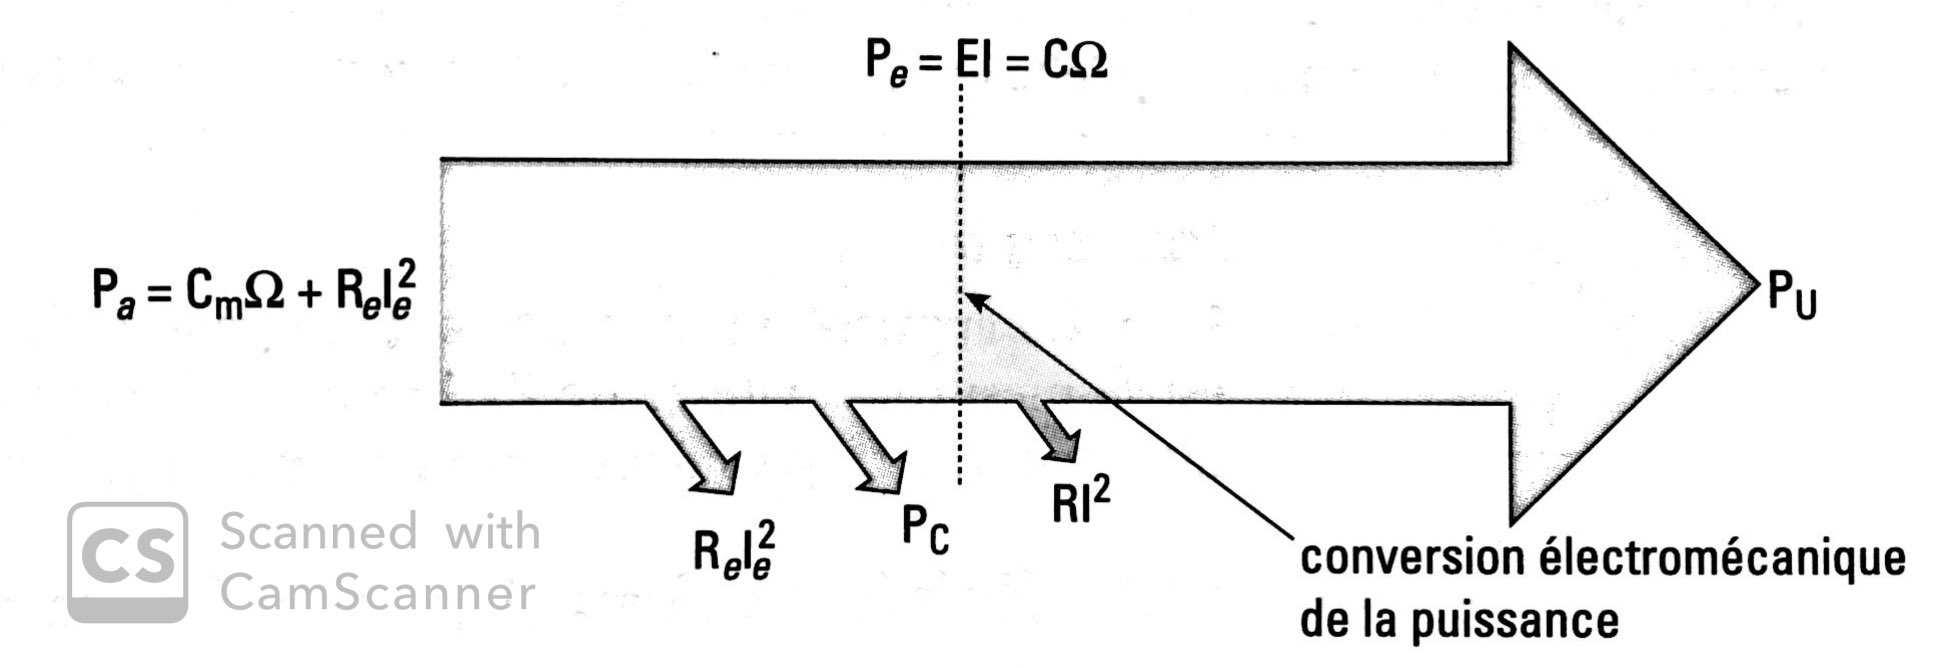
\includegraphics[scale=0.18]{puissanceg.jpg}
\end{center}



\subsubsection{Schéma fonctionnel du moteur en régime variable}
Lorsqu'il s'agit de prévoir le comportement de la machine en régime transitoire alors qu'elle évolue d'un premier point à un nouveau point de fonctionnement, la théorie des asservissements semble la plus appropriée pour traiter les variations d'état de la machine. Il s'agit de décrire les variations de grandeurs électriques et mécaniques autour d'un point de fonctionnement. Nous supposerons que le couple lié au frottements internes à la machine est proportionnel à la vitesse de rotation $\Omega$. Nous noterons $f$ le coefficient de frottement associé. On note aussi $-C_r$ le moment du couple résistant exercé sur l'axe de la machine. 
\medskip
En utilisant le théorème du moment cinétique :
\begin{equation}
    J \frac{d\Omega}{dt} = \sum C_i
\end{equation}
et en en faisant la transformée de Laplace
\begin{equation}
    Jp\Omega(p) = C(p) - f\Omega(p) - C_r(p)
\end{equation}
avec $C(p) = \Phi_0 I(p)$. On obtient alors :
\begin{equation}
    \Omega (p) = \frac{1}{f + Jp}(C(p) - C_r(p))
\end{equation}

Cette relation montre que la vitesse de la machine est la sortie d'un filtre passe bas d'ordre un, de constante de temps mécanique $\tau_m = \frac{J}{f}$ et dont l'entrée est la grandeur $C(p) - C_r (p)$.\medskip

L'équation électrique de l'induit ($U(t) = E(t) + RI(t) + L \frac{dI (t)}{dt}$) conduit par ailleurs à la relation :

\begin{equation}
    U(p) = E(p) + RI(p) + RpI(p) 
\end{equation}
avec $E(p)=\Phi_0 \Omega(p)$. Nous obtenons donc :

\begin{equation}
    I(p) = \frac{1}{R + Lp}(U(p) - E(p))
\end{equation}

Cette relation montre que l'intensité du courant traversant l'induit est la sortie d'un second filtre passe-bas d'ordre 1, de constante électrique $\tau_e = \frac{L}{R}$ et dont l'entrée est la grandeur $U(p) - E(p)$.

\begin{center}
    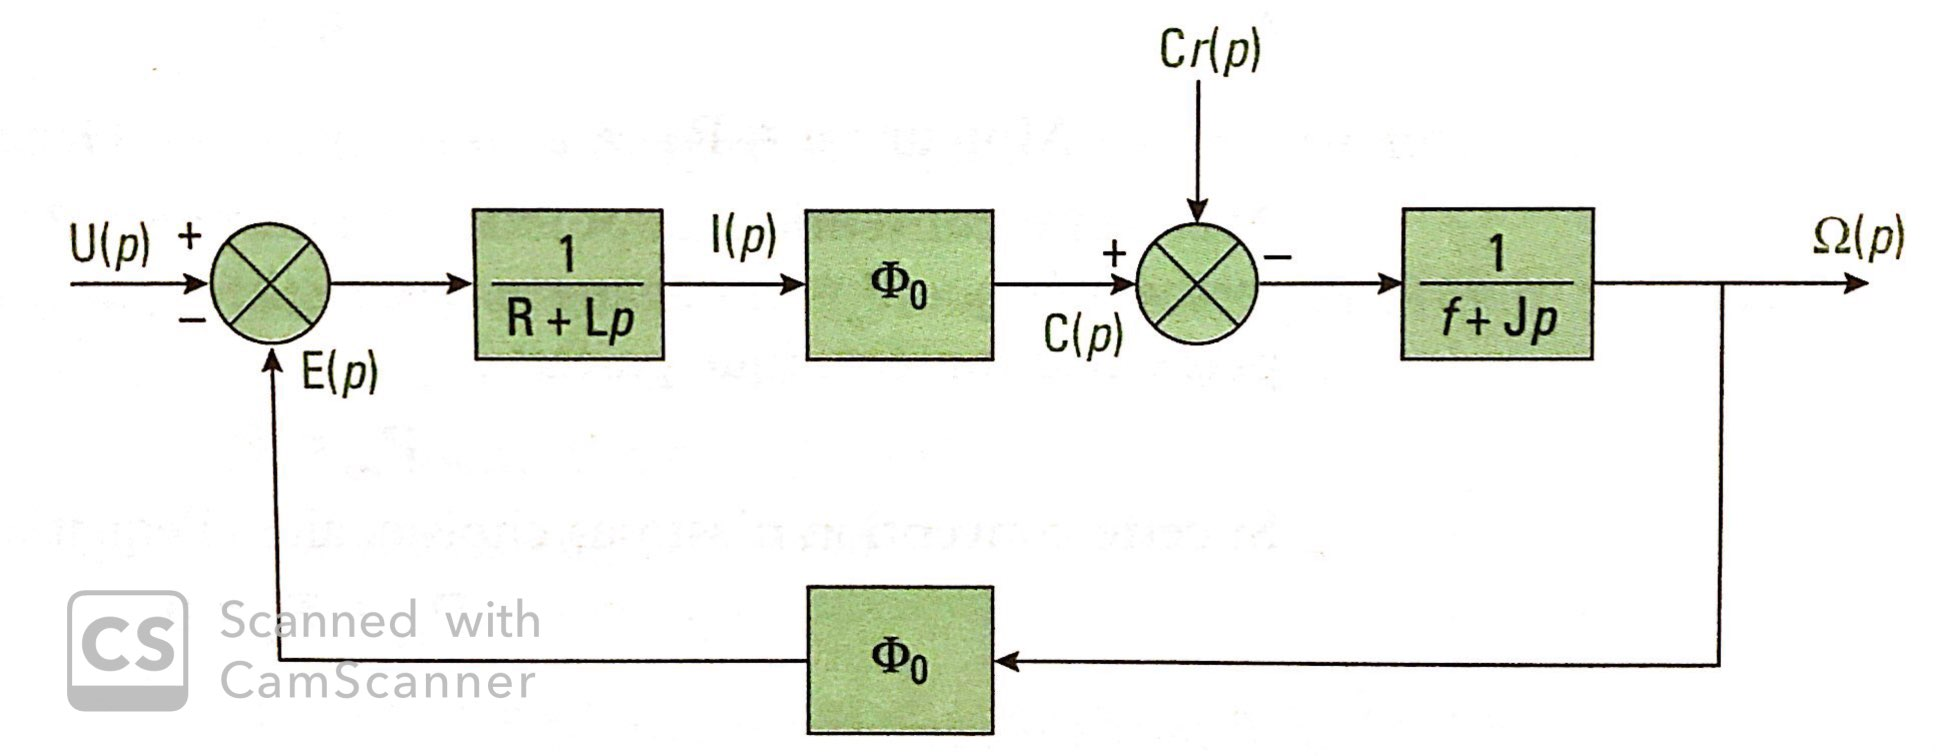
\includegraphics[scale=0.18]{schemabloc2.jpg}
\end{center}


\textcolor{blue}{Conclusion MCC : Les moteurs à courant continu ont été longtemps les champions de la vitesse réglable. La régulation de la vitesse et les asservissements de vitesse et de position ont été maîtrisés pour les moteurs à courant continu bien avant les autres types de moteurs.}\medskip

\textcolor{blue}{A puissance égale, les moteurs à courant continu sont beaucoup plus coûteux que les moteurs asynchrones (bobinages au stator et au rotor, collecteur, balais). Le système balais-collecteur est fragile, il nécessite surveillance et entretien. Par exemple, les moteurs TGV Paris-Sud-Est doivent subir un démontage complet et un reprofilage du collecteur tous les $300.000$ km, grosso modo, tous les ans. Les moteurs à courant continu sont donc actuellement réservés aux usages qu'ils sont les seuls à pouvoir satisfaire.}\medskip

\textcolor{blue}{Néanmoins, les applications pour l'automobile, restent un grand marché pour les moteurs à courant continu : démarreur, refroidisseur du moteur thermique, pompe à carburant, essuie-glace, lève-vitre, ventilateur, climatiseur... etc}\medskip






\section{Machines à courant alternatif}

%La machine synchrone est un exemple de convertisseur électromagnétique réversible, fonctionnant en moteur ou en générateur. Les alternateurs, machines synchrones génératrices, sont utilisés dans la production d'énergie électrique sous forme de courant alternatif ou bien dans des applications de moindre puissance plus courantes comme, par exemple, les véhicules automobiles.\medskip

%Le moteur synchrone qui présentait des difficultés d'adaptabilité en vitesse est désormais d'utilisation beaucoup plus souple grâce aux interfaces de commandes électroniques de puissance qui lui permettent de fonctionner en vitesse variable. A l'heure actuelle, le moteur synchrone autopiloté, et le moteur brushless, machine synchrone autopilotée à aimant permanent, c'est à dire l'ensemble formé par le moteur muni de tout le dispositif électronique de commande, sont très largement utilisés dans l'industrie et pour la traction que ce soit pour la motorisation des modèles réduits, des vélos à assistance électrique, des véhicules hybrides ou des TGV.

% Parler aussi des machines asynchrones

Pour toute machine alternative, on cherche à créer un champ magnétique tournant au niveau du stator qui permettra de mettre en rotation un rotor. 

\subsection{Réalisation d'un champ magnétique tournant}
On considère une aiguille aimantée située entre deux bobines identiques face-à-face et connectées en série, à égale distance de celles-ci. Les bobines sont alimentées par un signal sinusoïdal de pulsation $\omega$ qui engendre un champ magnétique sinusoïdal, variable dans le temps, au niveau de l'aiguille aimantée. 


\begin{center}
    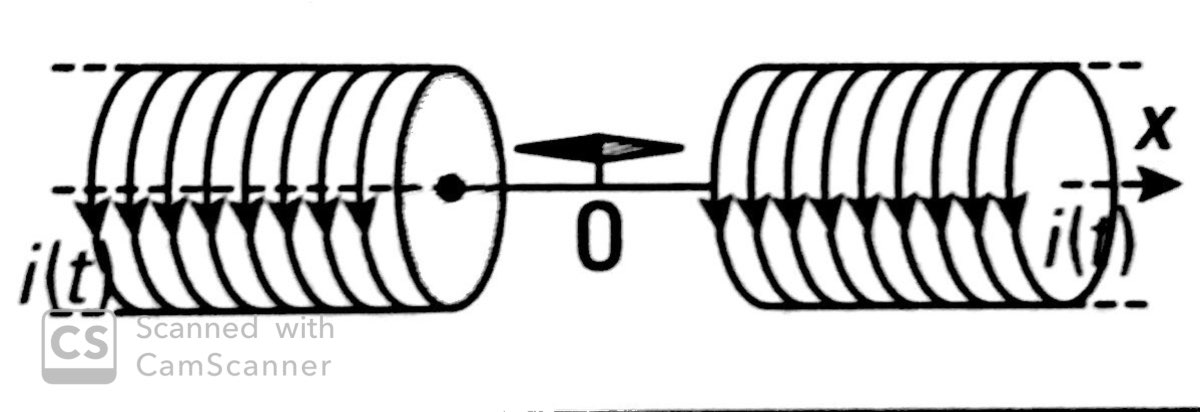
\includegraphics[scale=0.18]{2bobinesface.jpg}
\end{center}


L' aiguille vibre légèrement mais ne tourne pas, une légère impulsion est nécessaire pour la faire tourner (dans le sens de l'impulsion) à une vitesse $\omega$ égale à la pulsation du courant traversant la bobine. On dit qu'elle tourne au sychronisme. 

On comprend alors mieux la nécessité d'un champ tournant qui permettrait d'un côté de contrôler dans quel sens on démarre le moteur et d'un autre côté de démarrer le moteur sans intervention extérieure. 

\medskip

Pour créer un champ tournant, nous pouvons utiliser deux bobines placées à 90$^\circ$ dont le courant est déphasé de $\frac{\pi}{2}$. 

\begin{center}
    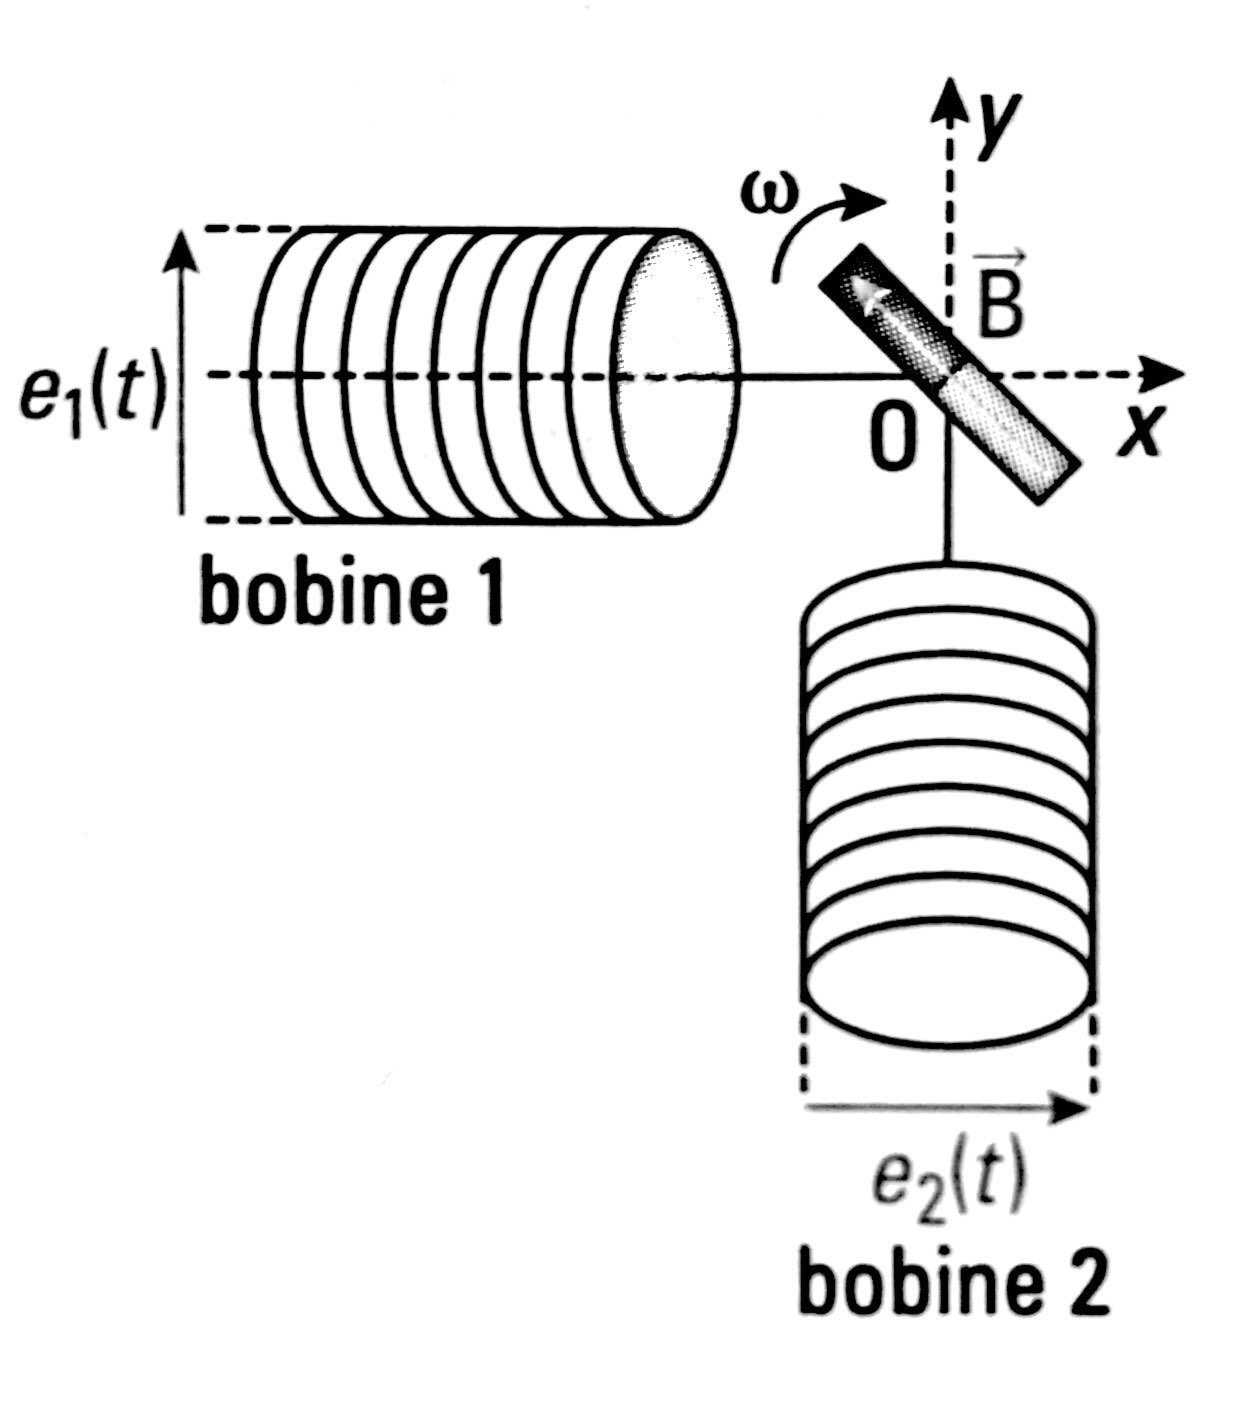
\includegraphics[scale=0.14]{bobinesdiphasees.jpg}
\end{center}

Un champ magnétique tournant est un champ de norme constante dont la direction varie dans un plan avec une vitesse angulaire $\omega$ constante. On l'écrit : 
\begin{equation}
    \vec{B} = B_0 cos(\omega t)\vec{u_x} + B_0 sin(\omega t)\vec{u_y}
\end{equation}

Les machines alternatives possèdent en règle générale plusieurs pôles. Si le stator possède $p$ paires de pôles, la rotation du rotor s'effectue alors à la vitesse $\frac{\omega}{p}$, dans le cas des machines synchrones, où $\omega$ est la pulsation du courant créant le champ tournant.

\subsection{Principe du moteur synchrone}

Le moteur synchrone est constitué d'un rotor à aimants permanents ou un électroaimant à courant continu. Le rotor crée un champ magnétique que l'on peut assimiler au champ créé par un aimant permanent.\medskip

Le stator est constitué de bobinages qui sont alimentés par un courant alternatif Ces bobinages produisent un champ magnétique tournant et à répartition spatiale sinusoïdale le long de l'entrefer.\medskip

Le champ tournant est noté :

\begin{equation}
    \vec{B} = B_0 \cos(\omega t + \theta_0)\vec{u_x} + B_0 \sin(\omega t + \theta_0)\vec{u_y}
\end{equation}

où $\theta_0$ représente l'angle entre le champ tournant et le moment magnétique $\vec{M}$ à l'instant $t=0$.\medskip

Le rotor est considéré en rotation dans le plan $(Oxy)$. Notons :
\begin{equation}
    \vec{M} = M_0 \cos(\Omega t) \vec{u_x} + M_0\sin(\Omega t )\vec{u_y}
\end{equation}
où $\Omega$ représente la vitesse de rotation du rotor.\medskip

Le rotor subit un couple engendré par le champ tournant de la forme $\vec{\Gamma} = \vec{M} \land \vec{B}$. Soit ici :
\begin{equation}
    \vec{\Gamma} (t) = M_0 B_0 [\cos(\Omega t)\sin(\omega t + \theta_0) - \sin(\Omega t)\cos(wt+\theta_0)] \vec{u_z} = M_0 B_0 \sin ((\omega - \Omega)t + \theta_0) \vec{u_z}
\end{equation}

Cette équation ne permet pas d'interpréter à elle seule les observations expérimentales

\textbf{Expérience et interprétation}\medskip

Experimentalement :\medskip

- Lorsque le moteur synchrone est directement alimenté par une tension de fréquence $50 Hz$, celui-ci ne démarre pas.\medskip

- En réduisant la fréquence, le moteur démarre à des fréquences faibles. On peut ensuite augmlenter la fréquence jusqu'à $50 Hz$ sans que le moteur s'arrête de tourner.\medskip

- La constante de temps mécanique $\tau$ du moteur est important devant la période de la tension d'alimentation. Cette inertie mécanique fait que la machine n'est sensible en réalité qu'à la valeur moyenne des grandeurs électriques si la pulsation est trop importante (comportement de type filtre passe-bas).\medskip


- Lorsque le moteur est à l'arrêt ($\Omega = 0$ et $\omega = 100 \pi rad.s^{-1}$),

\begin{equation}
    \langle \vec{\Gamma}(t) \rangle = M_0 B_0 \langle sin( \omega t + \theta_0 ) \rangle \vec{u_z} = \vec{0}
\end{equation}

Et le moteur ne démarre pas. Lorque la fréquence est diminuée, la période $T$ des grandeurs électriques (et donc du champ magnétique) se rapproche de $\tau$. A partir d'un certain seuil, le rotor est sensible à la valeur instantanée du couple et la machine se met à tourner à la vitesse angulaire $\Omega$. En régime permanent, le couple électromagnétique moyen exercé sur le rotor s'écrit :
\begin{equation}
    \langle \vec{\Gamma}(t) \rangle = M_0 B_0 \langle sin(\theta_0 ) \rangle \vec{u_z}
\end{equation}
puisqu'alors le rotor tourne au \textbf{synchronisme} ($\omega = \Omega$) d'où le nom de moteur \textbf{synchrone}.\medskip

D'après la valeur de $\langle \vec{\Gamma}(t) \rangle$, la valeur de $\theta_0$ influe sur le couple. Cet angle est considéré comme la variable dont dépend le couple, c'est à dire que la machine adapte cette valeur pour qu'en régime permanent il y ait égalité du couple moteur et du couple résistant s'exerçant sur la machine.\medskip

Le signe de $\theta_0$ permet de définir le mode de fonctionnement de la machine. Si $\theta_0$ est positif, il s'agit d'un couple moteur (B en avance par rapport à M). S'il est négatif, il s'agit d'un couple résistant (génératrice, M en avance par rapport à B).

\begin{center}
    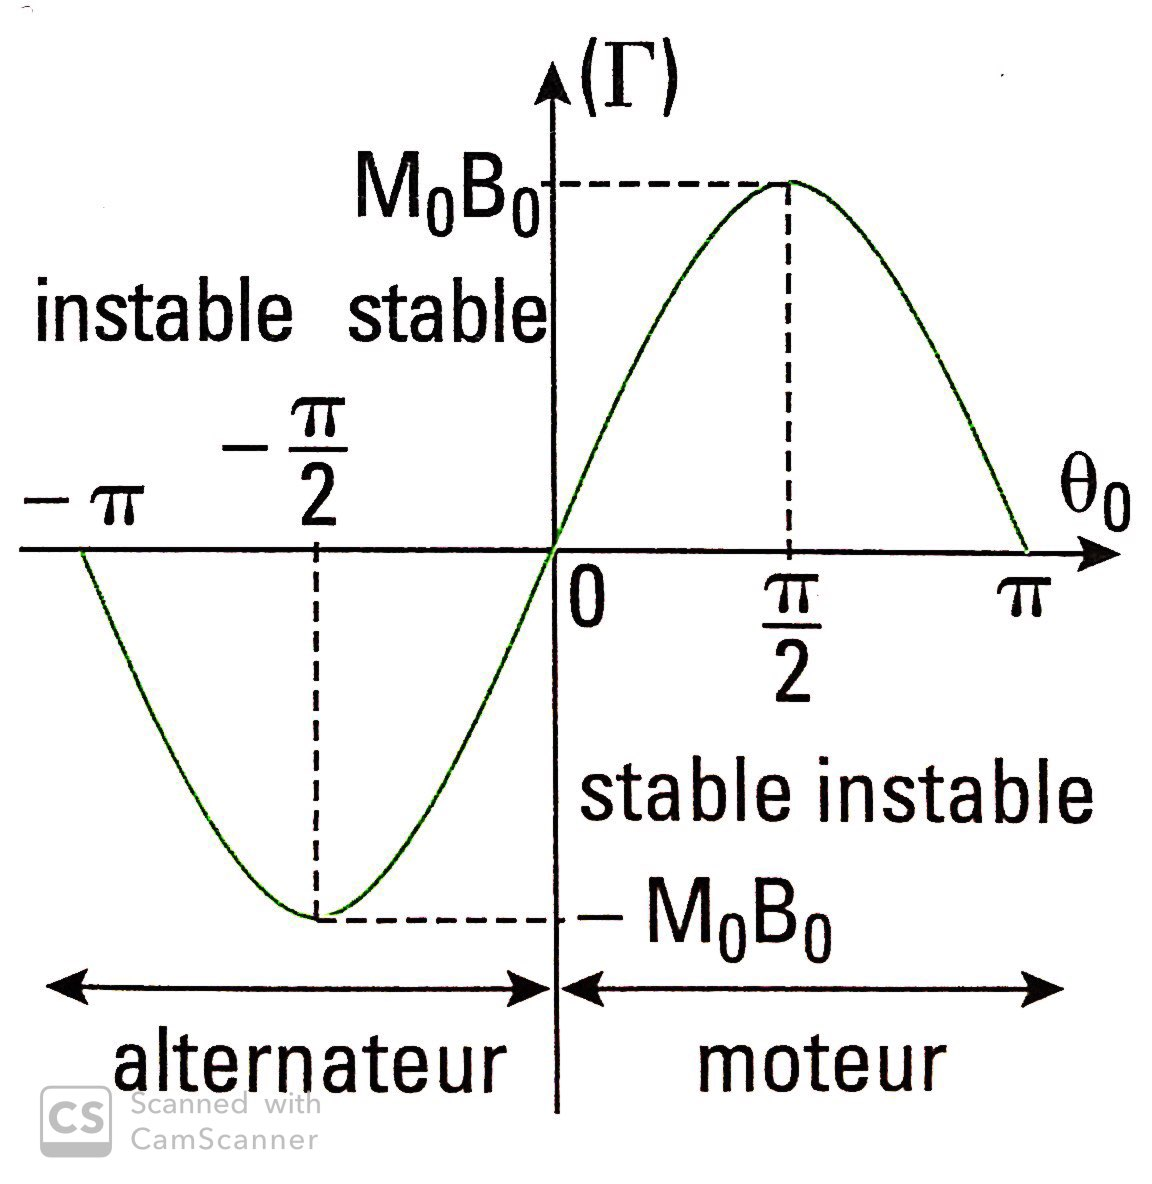
\includegraphics[scale=0.12]{theta0.jpg}
\end{center}

Suivant le mode de fonctionnement apparaissent une zone de fonctionnement stable et une zone instable.\medskip

Si lors du fonctionnement du moteur, le couple résistant devient, en valeur absolue, supérieur à $M_0B_0$, le moteur \textbf{décroche}, c'est à dire que ne pouvant pas fournir le couple nécessaire, il s'arrete.\medskip

Lorsque le moteur est soumis à un couple de charge $-\langle \vec{\Gamma}(t) \rangle$ inférieur à $M_0 B_0$, on obtient deux positions de fonctionnement $\theta_1$ et $\theta_2$ comme montre la figure.


\begin{center}
    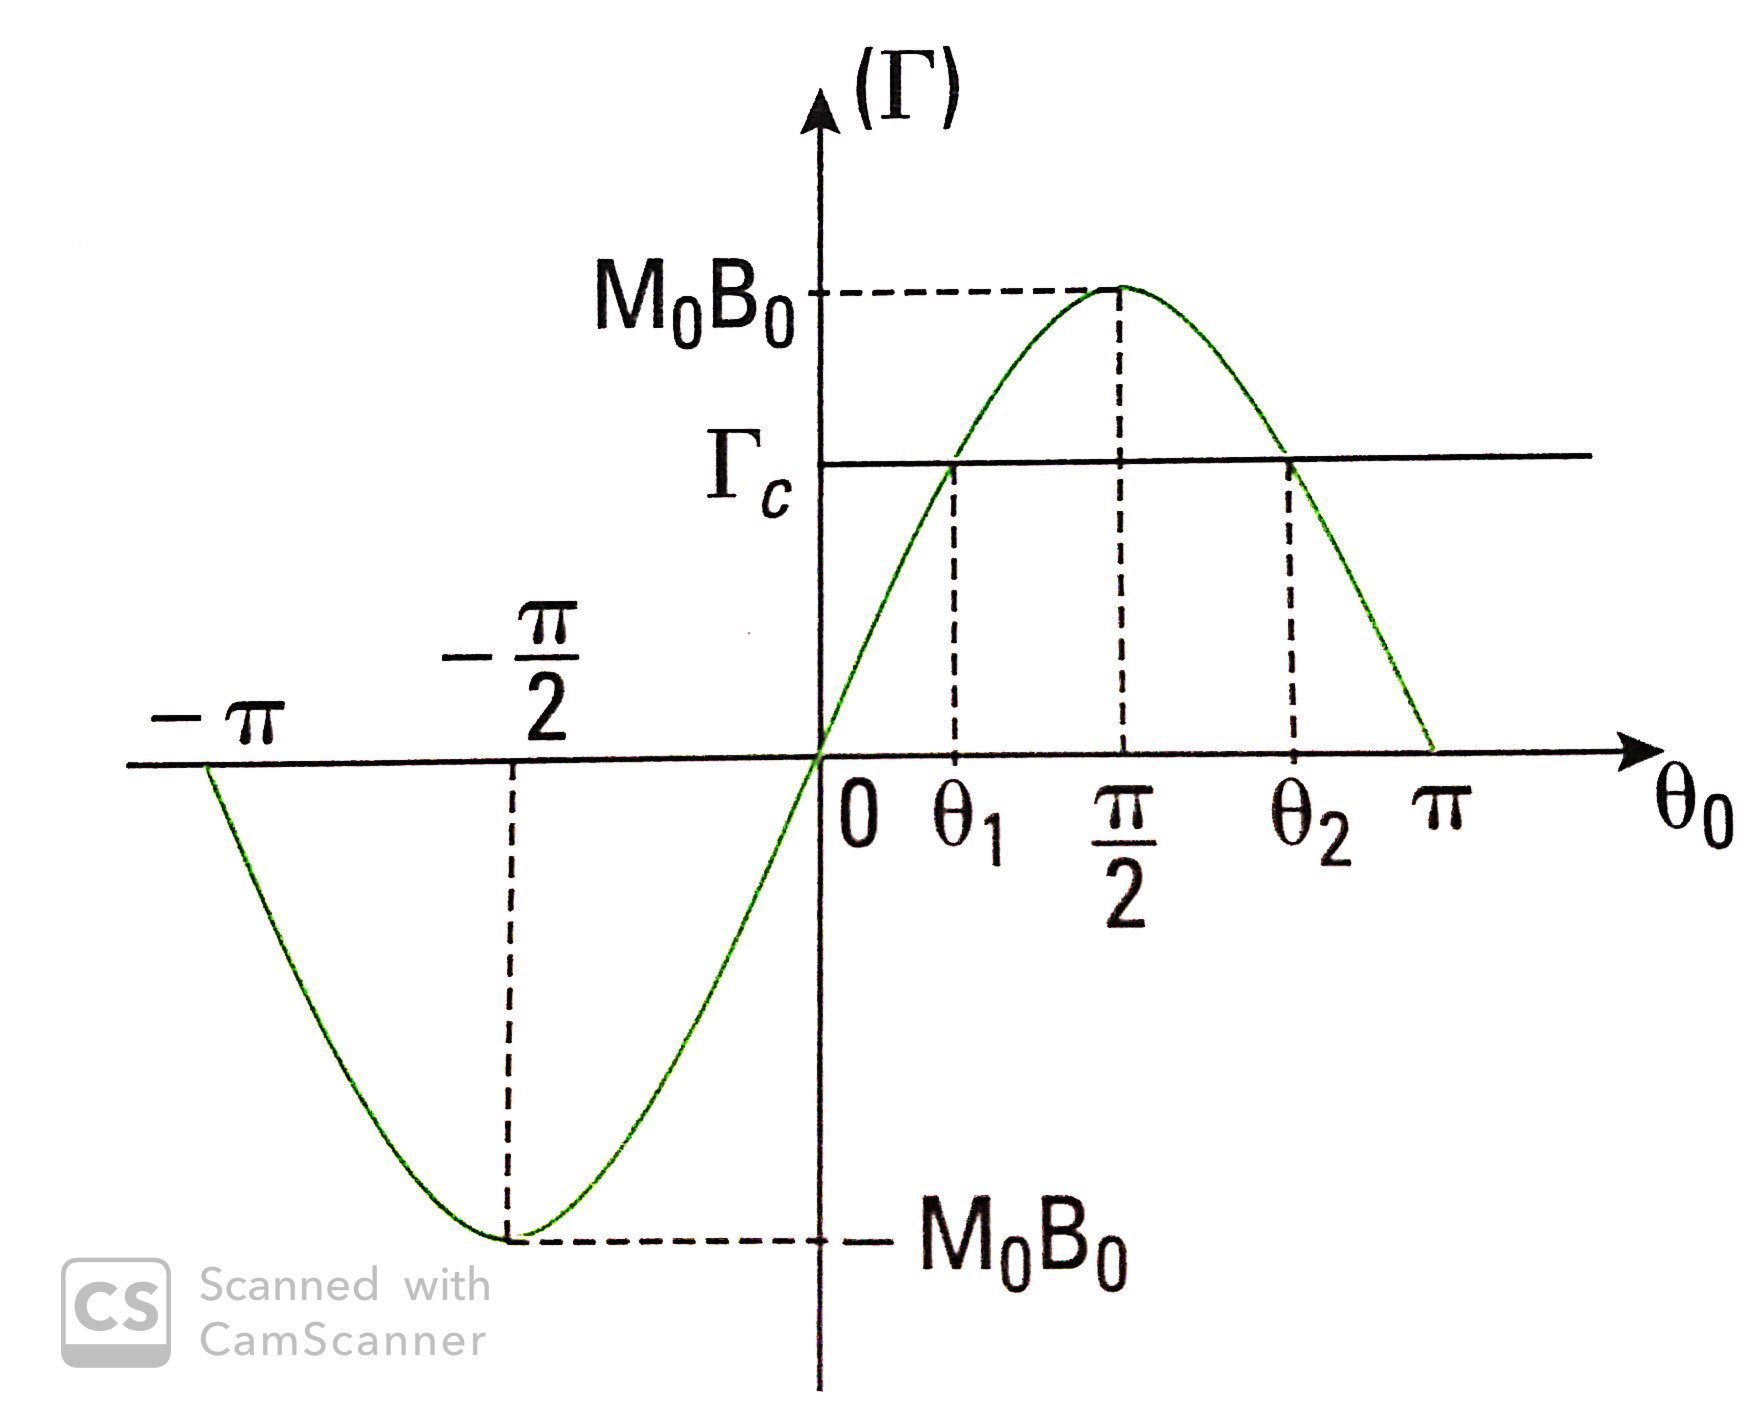
\includegraphics[scale=0.1]{theta12.jpg}
\end{center}


\begin{itemize}
    \item Pour $\theta_0 = \theta_1$ : si le moteur accélère, le moment magnétique tourne plus rapidement que le champ tournant et le rattrape, donc l'angle $\theta_0$ diminue. Si cet angle diminue, le graphe indique que le couple moteur diminue. Donc le moteur ralentit. Cette position d'équilibre est donc \textbf{stable}.
    \item Pour $\theta_0 = \theta_2$ : si le moteur accélère, le moment magnétique tourne plus rapidement que le champ tournant et le rattrape, donc l'angle $\theta_0$ diminue. Si cet angle diminue, le graphe indique que le couple moteur augmente, donc le moteur accélère. Cette position d'équilibre est donc \textbf{instable}.
\end{itemize}

\textcolor{blue}{Conclusion moteurs synchrones : Les moteurs synchrones sont appreciés pour leurs vitesse rigoureussement constante, liée à la fréquence du réseau, par exemple ils sont utilisés en tant que programmateurs dans les électroménagers (lave-linge, four,...). Pour les applications industrielles, le moteurs synchrones est resté longtemps marginal car il présente deux inconvénients quand il est alimenté directement par le réseau : il ne démarre pas spontanément; si la charge augmente trop, le rotor décoche (il cale brusquement et se met à vibrer).}\medskip

\textcolor{blue}{Dans les années 80, le développement des alimentations électroniques triphasées à fréquence réglable a révolutioné l'utilisation des moteurs synchrones, avec la génération des moteurs auto-pilotés. Dans ce type de moteurs, la fréquence des courants du stator est controlée par des capteurs mesurant en permanence la position du champ magnétique du rotor par rapport à la position du champ magnétique tournant. Les problèmes de démarrage et de décrochage sont alors résolus, et la vitesse devient réglable par une action extérieure sur la fréquence.}

\textcolor{blue}{Utilisés pour la motorisation des véhicules réduits, des vélos à asistance électrique, des véhicules hybrides ou des TGV.}

\subsection{Moteur Asynchrone}

Le bobinage du stator, alimenté en courant alternatif, produit un champ magnétique tournant dont la vitesse est fixée par la fréquence du courant et le nombre de pôles du bobinage. Dans le rotor en fer, sont inclus des conducteurs en aluminium coulé, parallèles à l’axe, leurs extrémités étant toutes reliées entre elles par des anneaux de même métal pour former ce qu’on appelle la \textbf{cage à écureuil}. Il n’y a aucun contact électrique entre le rotor et l’extérieur. Le mouvement du champ tournant provoque des courants induits dans la cage en aluminium du rotor, les forces de Laplace sur ces courants produisent la rotation.\medskip

\begin{tabular}{cc}
   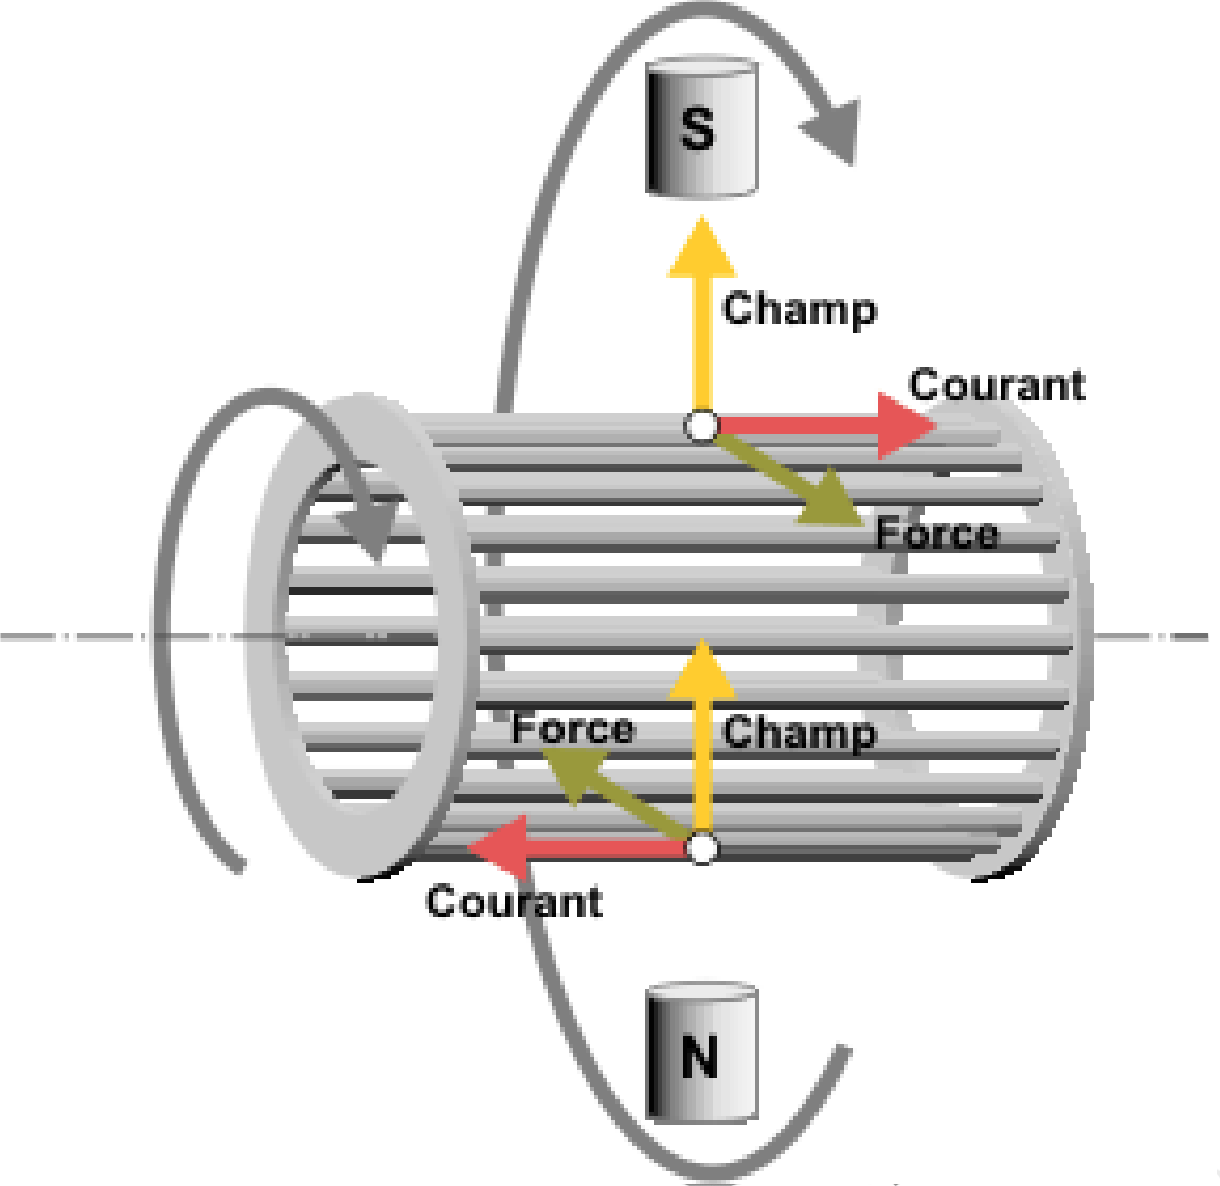
\includegraphics[scale=0.28]{asynchrone.png} &
   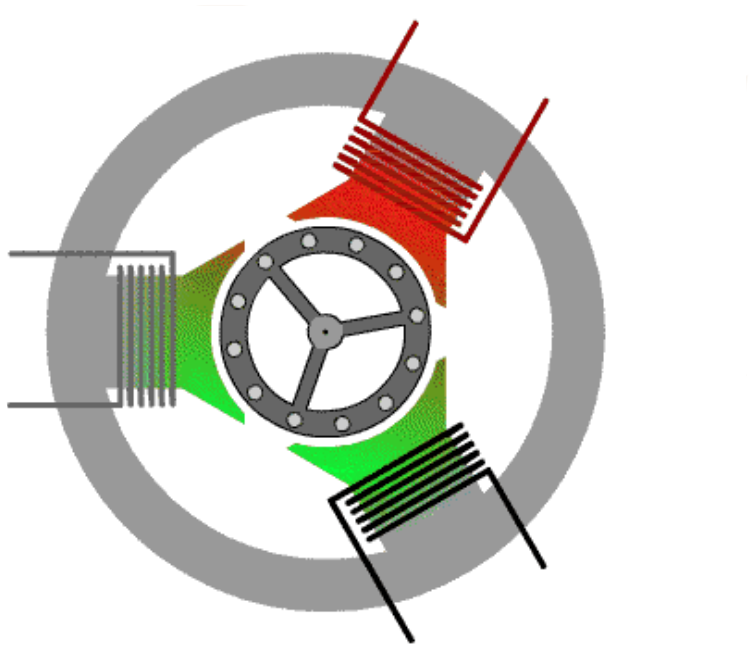
\includegraphics[scale=0.4]{asynchrone2.png} \\
\end{tabular}


\medskip

Le rotor peut être assimilé à un bobinage de résistance $R$, d'inductance propre $L$, comportant $N$ spires, de section $S$ et dans lequel on peut considérer le champ uniforme.\medskip

Le rotor tourne à la vitesse de rotation $\Omega$ et le champ tournant est de la forme :

\begin{equation}
    \vec{B} = B_0 cos(\omega t + \theta_0) \vec{u_x} + B_0 sin(\omega t + \theta_0 ) \vec{u_y}
\end{equation}

où $\theta_0$ représente l'angle entre le champ tournant et l'axe de la spire à $t=0$.

\begin{center}
    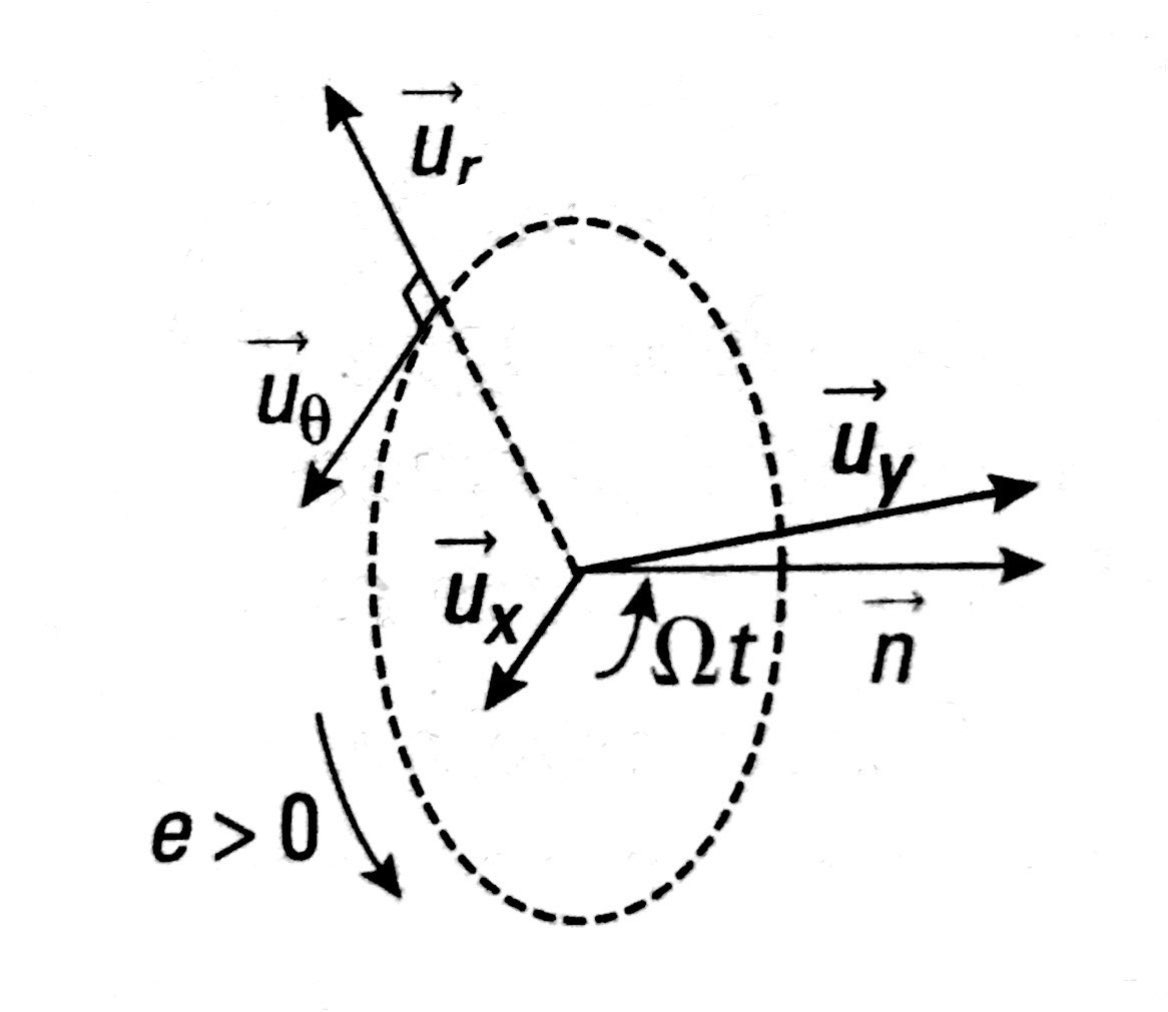
\includegraphics[scale=0.14]{spireasync.jpg}
\end{center}

Cette bobine est le siège d'une f.é.m calculée à partir de la loi de Faraday :
\begin{equation}
    e =- \frac{d\Phi}{dt} 
\end{equation}
où 
\begin{equation}
    \Phi = \vec{B} \cdot \vec{S}
\end{equation}

D'après la figure on a :

\begin{equation}
    \Phi = NS\vec{B} \vec{n}
\end{equation}

où $\vec{n} = cos(\Omega t) \vec{u_x} + sin(\Omega t)\vec{u_y}$ est le vecteur normal à la spire.

\begin{equation}
    e = - \frac{d}{dt} (NSB_0 (cos(\omega t + \theta_0)cos(\Omega t) + sin(\omega t +\theta_0) sin (\Omega t)))
\end{equation}
\begin{equation}
     e = - \frac{d}{dt} (NSB_0 cos((\omega -\Omega)t + \theta_0) = (\omega - \Omega)NSB_0 sin((\omega -\Omega)t + \theta_0)
\end{equation}

Cette f.é.m présente dans le bobinage en circuit fermé engendrant l'apparition d'un courant induit $i$. Elle est sinusoîdale et de pulsation $\omega -\Omega$. Nous pouvons alors utiliser la notation complexe pour définir ce courant induit. \medskip

Le bobinage peut être modélisé comme dans la figure suivante :

\begin{center}
    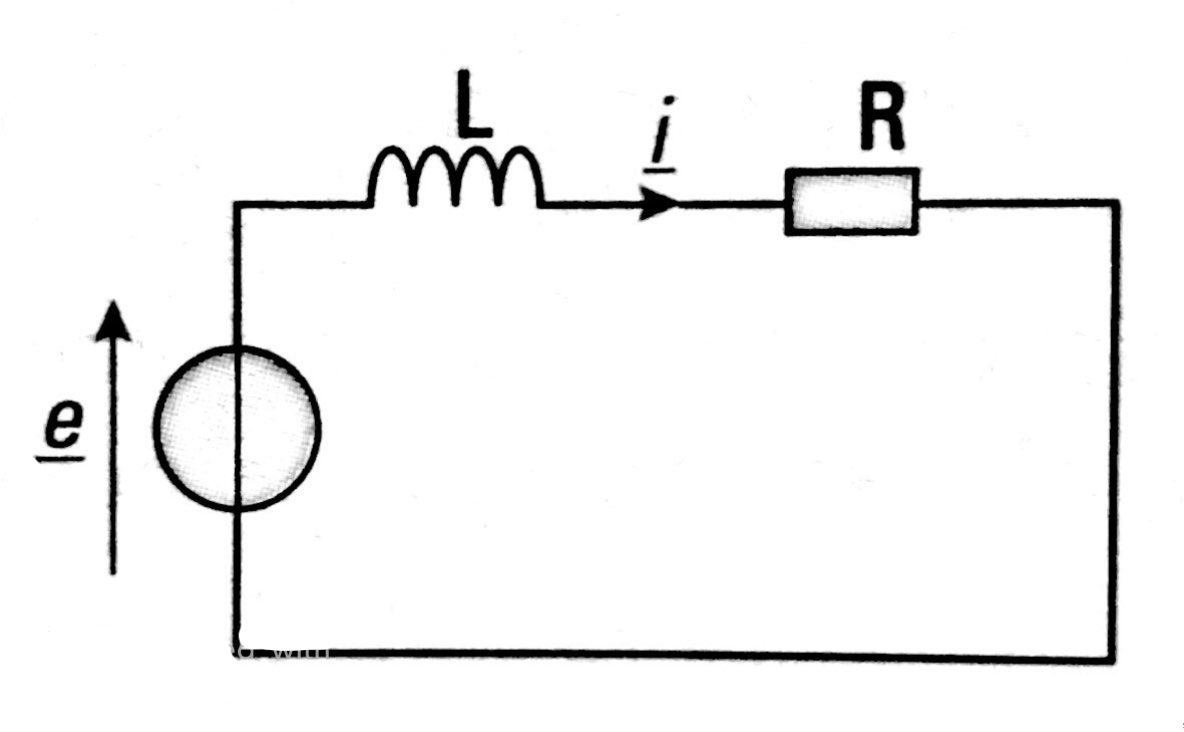
\includegraphics[scale=0.1]{RLasync.jpg}
\end{center}
 
\begin{equation}
    \underline{e} = (R + jL(\omega - \Omega)) \underline{i}
\end{equation}
d'où
\begin{equation}
    i = \frac{(\omega - \Omega)NSB_0}{\sqrt{R^2-L^2(\omega - \Omega)^2}} sin\left ( (\omega - \Omega)t + \theta_0 - Arctan \left ( \frac{L (\omega - \Omega)}{R} \right ) \right )
\end{equation}

On supose par la suite $\varphi = Arctan \left ( \frac{L (\omega - \Omega)}{R} \right )$.

Le bobinage parcouru par le courant $i$ est assimilé à un moment magnétique :
\begin{equation}
    \vec{M} = NSi\vec{n} = NSi(cos(\Omega t) \vec{u_x} + sin(\Omega t)\vec{u_y})
\end{equation}

$\vec{M}$ subit un couple engendré par le champ tournant de la forme $ \vec{\Gamma} = \vec{M} \land \vec{B} $. D'où :

\begin{equation}
    \vec{\Gamma}(t) = NSiB_0(cos(\Omega t) sin(\omega t + \theta_0) - sin(\Omega t)cos(\omega t + \theta_0))\vec{u_z}
\end{equation}

Or $cos(\alpha)sin(\beta) - sin(\alpha)cos(\beta) = sin(\beta - \alpha)$, donc :

\begin{equation}
    \vec{\Gamma}(t) = NSiB_0 sin ((\omega - \Omega) t + \theta_0) \vec{u_z}
\end{equation}

D'où :

\begin{equation}
     \vec{\Gamma}(t) = \frac{(\omega - \Omega)(NSB_0)^2}{\sqrt{R^2+L^2(\omega - \Omega)^2}} sin((\omega - \Omega) t + \theta_0 - \varphi)sin((\omega - \Omega) t + \theta_0))\vec{u_z}
\end{equation}

Or, $2sin(a)sin(b) = cos(a - b) - cos(a+b)$, ce qui donne :

\begin{equation}
     \vec{\Gamma}(t) = \frac{(\omega - \Omega)(NSB_0)^2}{2\sqrt{R^2+L^2(\omega - \Omega)^2}} (cos(\varphi) - cos (2(\omega - \Omega) t + 2 \theta_0 - \varphi))\vec{u_z}
\end{equation}

De même que pour la machine synchrone, le rotor, du fait de son inertie, n'est sensible qu'à la valeur moyenne du couple, c'est à dire :

\begin{equation}
    \langle \vec{\Gamma}(t) \rangle = \frac{(\omega - \Omega)(NSB_0)^2}{2\sqrt{R^2+L^2(\omega - \Omega)^2}} cos(\varphi) \vec{u_z}
\end{equation}

On pose : $(\omega - \Omega) = g\omega$, où $g$ est appelé le glissement.\medskip

De plus, $cos(\varphi) = \sqrt{\frac{1}{1 + tan^2 (\varphi)}}= \frac{R}{\sqrt{R^2 + L^2(\omega -\Omega)^2}}$ , soit :

\begin{equation}
     \langle \vec{\Gamma}(t) \rangle = \frac{g\omega (NSB_0)^2R}{2(R^2 + g^2L^2\omega^2)}\vec{u_z}
\end{equation}

Contrairement au moteur synchrone, le moteur asynchrone possède un couple nul au synchronisme (g=0). Il tourne donc à une vitessz différente de la pulsation d'alimentation, d'où sa denomination, moteur asynchrone.\medskip

En règle générale, la valeur du glissement est faible et le rotor tourne à une vitesse de rotation proche de la valeur de pulsation. La valeur du glissemnt dépend de la charge mécanique (tout comme l'angle $\theta_0$ du moteur synchrone dépend de la charge).\medskip

Remarquons que le couple de démarrage, obtenu pour $g=1$, est non nul :

\begin{equation}
    \langle \vec{\Gamma}(t) \rangle = \frac{\omega (NSB_0)^2R}{2(R^2 + L^2\omega^2)}\vec{u_z}
\end{equation}


\begin{center}
    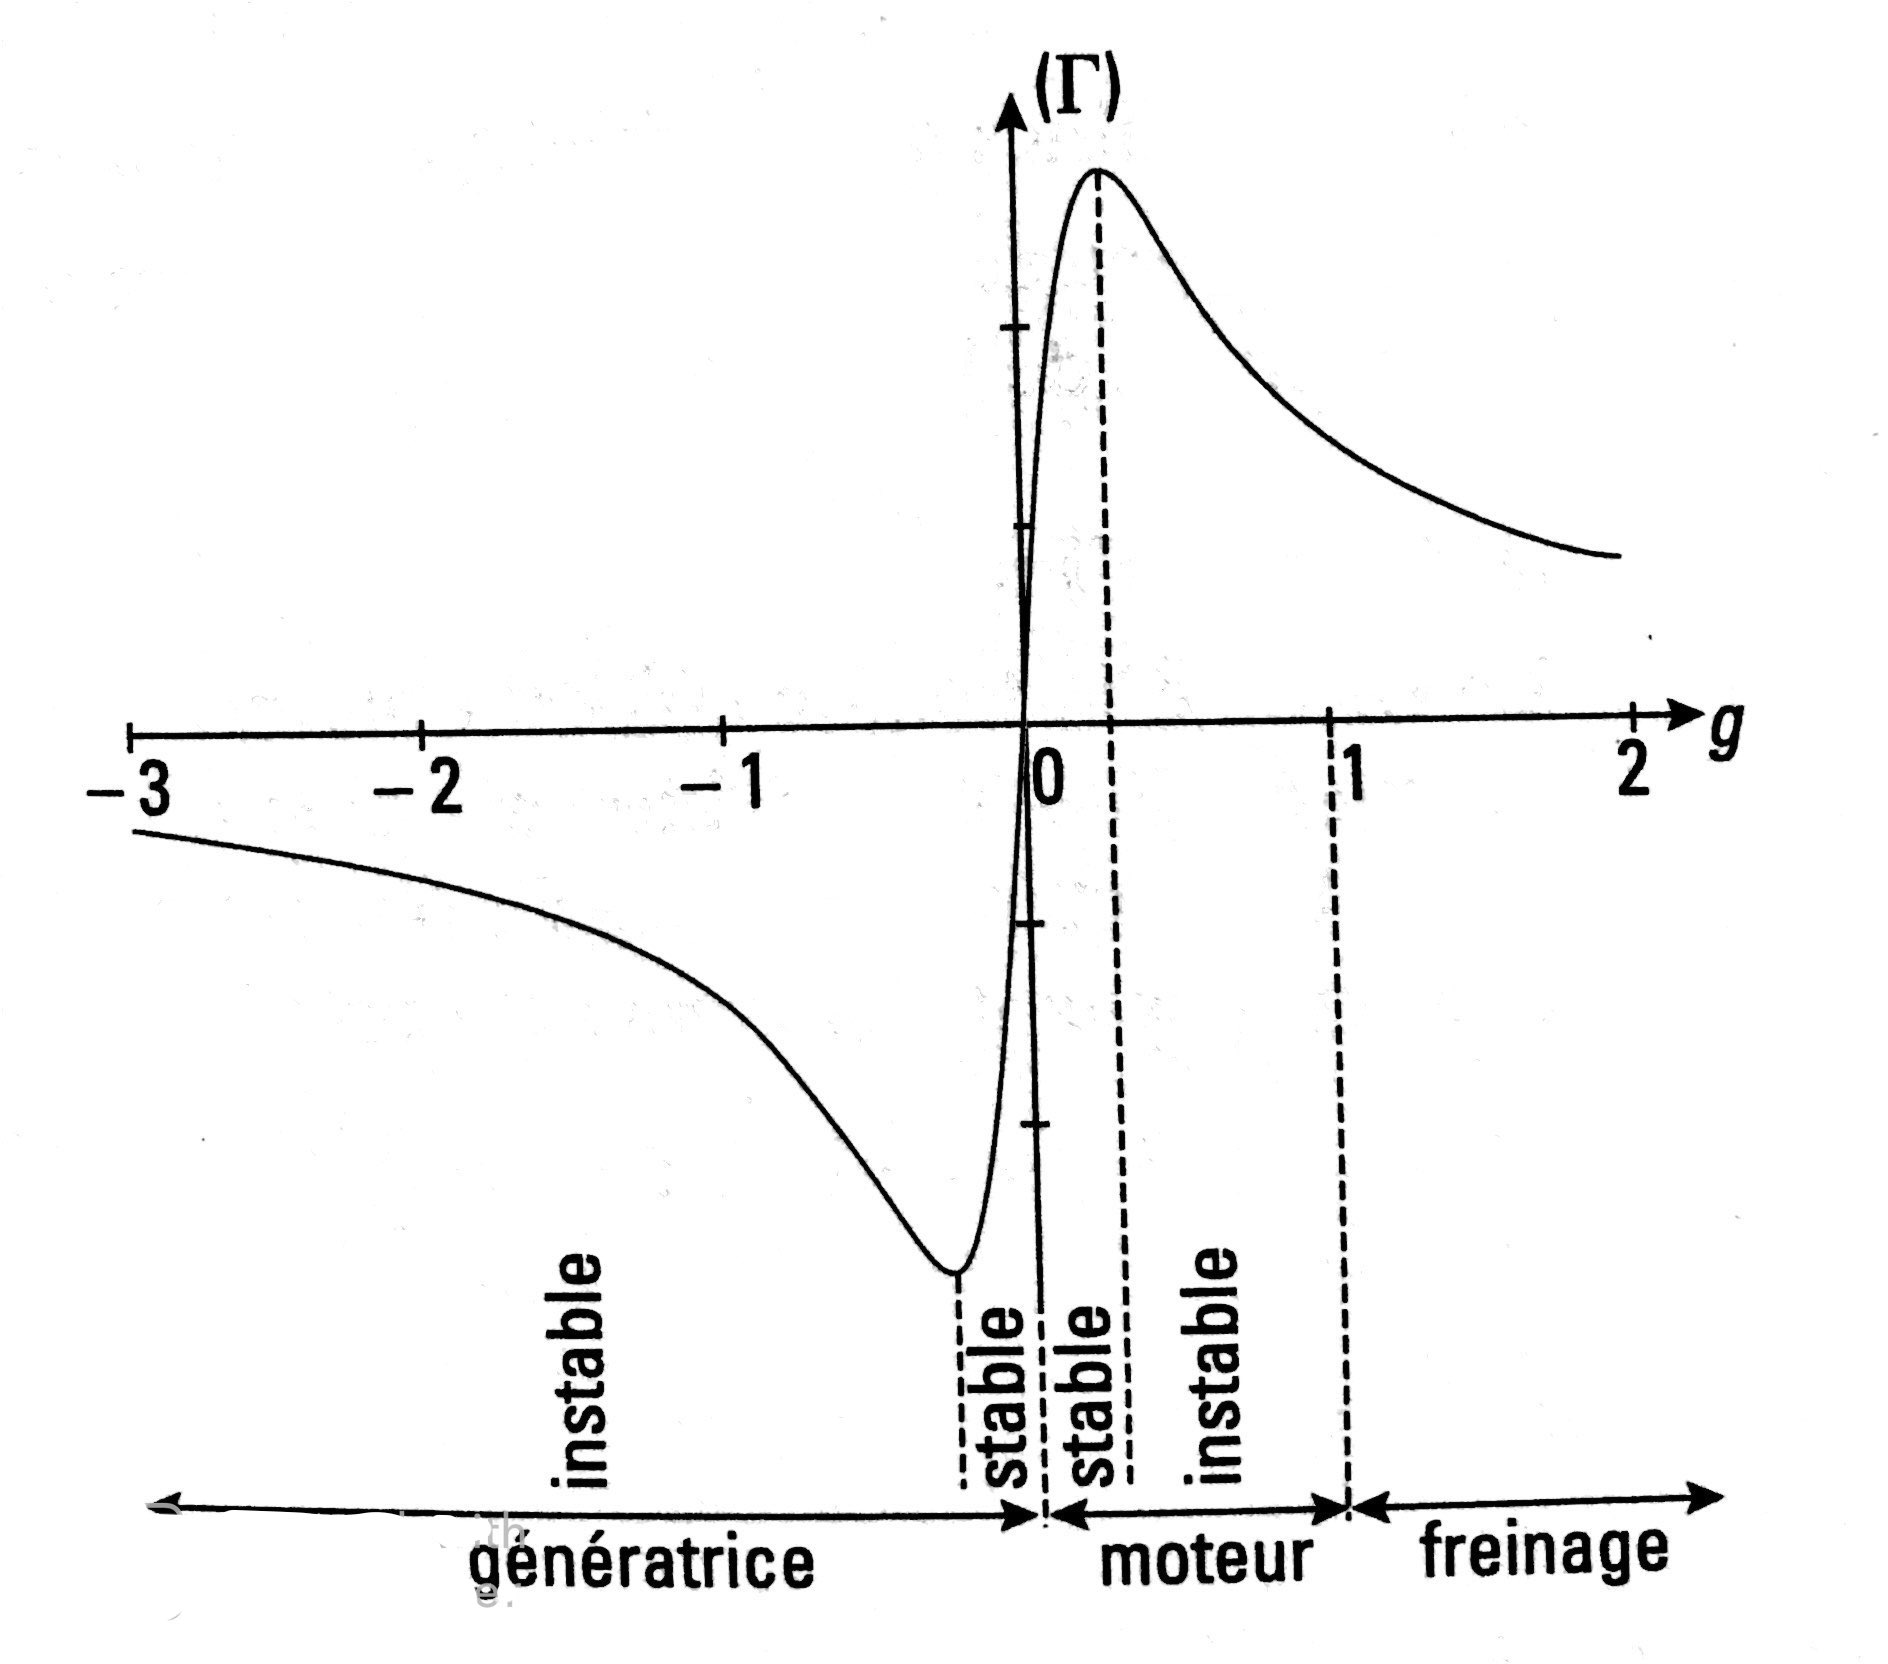
\includegraphics[scale=0.12]{graphasync.jpg}
\end{center}



Sur la figure on obserbe :

\begin{itemize}
    \item Lorsque la vitesse de rotation est positive et le couple positif, la machine fonctionne en moteur puisque l'étude est réalisée en convention récepteur : ce qui correspond à la zone $g \in (0,1)$.
    \item Lorsque la vitesse de rotation est négative (rotation du rotor en sens inverse du champ tournant) et le couple moyen positif, le couple est résistant et freine la machine : c'est ce qui correspond à la zone $g > 1$. Une étude détaillé dans cette zone montre que la machine ne peut fournir aucune puissance électrique à l'extérieur Il ne s'agit donc pas d'un comportement génératrice. La machine fonctionne en mode freinage.
    \item Lorsque la vitesse de rotation est positive et supérieure à la pulsation du champ tournant et le couple négatif, la machine fonctionne en génératrice : c'est ce qui correspond à la zone $g<1$
\end{itemize}

Nous remarquons que le moteur asynchrone possède un couple maximal et que la zone de fonctionnement stable est réduite. Nous vérifions ainsi que le glissemnt doit être faible en régime établi.\medskip


\textcolor{blue}{Conclusion asynchrone : Les moteurs asynchrones triphasés sont très utilisés dans l'inductrie car il sont bon marché, robustes et sans entretien. Branchés directement au réseau triphasé, sa vitesse varie seulement de quelques pour cent entre le fonctionnement à vide et à plein charge, restant toujours un peu plus faible que la vitesse du champ magnétique tournant. De la même façon que pour les moteurs asynchrones, jusqu'aux années 80 le moteur asynchrone n'était pas utilisable pour les applications en vitesse variable. Actuellement, l'électronique de puissance permet de produire des tensions triphasées à fréquence variable.}


\section*{Conclusion}

\begin{center}
    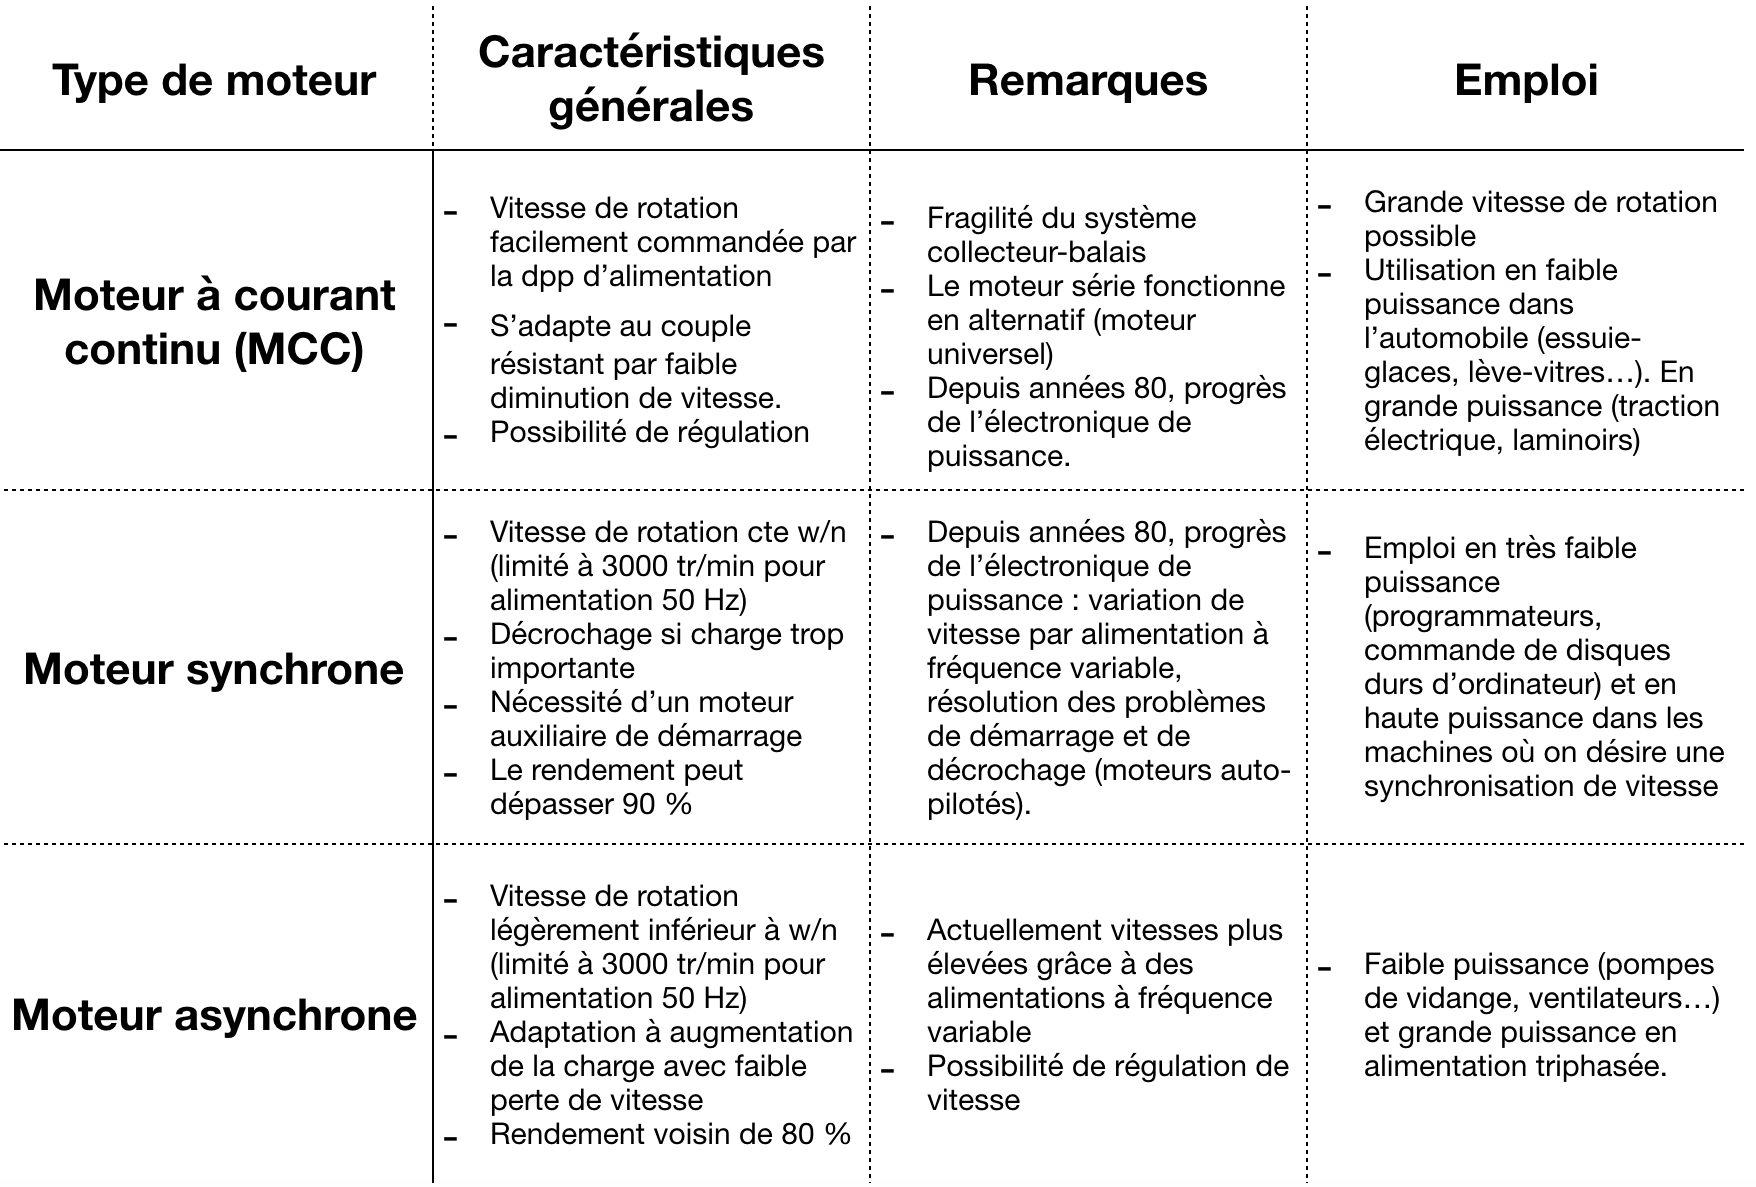
\includegraphics[scale=0.5]{Conclusiontableau.png}
\end{center}

\section*{Questions que je me pose}
\begin{itemize}
    \item Transformateur
    \item Alternateur
    \item Dynamo : génératrice à courant continu, inventé par Zénobe Théophile Gramme (1826-1901)
    \item avantages et inconvénients de la machine à courant continu par rapport aux moteurs synchrones et asynchrones.
    \item montage hacheur
    \item galvanomètre : mesure le courant induit
    \item différence entre force de Lorentz et force de Laplace
    \item moteur universel
    \item moteur pas à pas
    \item xq toute la puissance est dissipée par effet Joule dans l'inducteur de la MCC ? 
    \item sens courant induit dans la cage à écureuil ? 
\end{itemize}

\section*{Questions}
Dans la machine à courant continu, où passe le gros la puissance électrique ?\\
Dans l'induit = dans le rotor (on le voit parce que le couple est proportionnel au courant traversant l'induit).\\

Même question pour une machine synchrone ?\\
Dans le stator cette fois.\\

Dans le cas du moteur à courant continu, à quoi est due la résistance de l'induit ?\\
C'est essentiellement la résistance du bobinage.\\

Qu'est ce qui fait alors que cette résistance est faible ?\\
C'est l'intensité traversant l'induit qui fixe la section minimale des spires, permettant d'avoir une faible résistance.\\

Comment peut on limiter le courant de démarrage sans hacheur ?\\
On met un rhéostat de démarrage.\\

Dans le cas d'un moteur synchrone, comment déphase t-on les alimentations des différentes bobines ?\\
En utilisant un condensateur en série.\\

Quel est l'inconvénient de la machine synchrone ?\\
Elle ne démarre pas spontanément, et la vitesse est imposée par la fréquence du réseau.\\

Quel est l'ordre de grandeur du glissement pour un moteur de bateau par exemple ?\\
Quelques pour cents $\simeq 5\%$.\\

Faut il feuilleter le rotor dans une machine asynchrone ?\\
Le champ perçut par le rotor tour à la fréquence $\Omega_S-\Omega$ : très faible puisque $g\simeq 5\%$, donc il n'y a pas besoin de feuilleter car il y a très peu de pertes fer.

\section*{Remarque}
représenter plutôt C en fonction de $\Omega$.\\
Il faut préciser qu'on peut couper l'alimentation de l'induit, mais après avoir coupé celle de l'inducteur.\\

Il faut faire apparaître le lien entre fréquence et nombre de paire de pôles pour les moteurs synchrones.\\

Faire la distinction entre $\Omega_S$ : vitesse de rotation du champ statorique et $\Omega$ la vitesse de rotation du rotor.\\

On appelle souvent machine à induction les machines asynchrones.\\




\end{document}

